\documentclass[11pt, twoside, a4paper, titlepage, openany]{article}   	% {} --> Class: article, report, book, slides
										% [] --> Options: 
										% 11pt = size of the font
										% a4paper, a5paper, letterpaper (default)		
										% titlepage, notitlepage
										% onecolum, twocolumn
										% twoside, oneside = fronteretro o no
										% landscape = foglio orizzontale
								
\usepackage[binding=5mm]{layaureo}		% Layout pi� espanso preimpostato (bindings = spazio rilegatura)
%\usepackage[options]{geometry}             	% Layout completamente configurabile
							
\pagestyle{plain}						% plain (default)     :	stampa i numeri di pagine a pi� di pagina nel mezzo. 
									%		           
									% headings            :	stampa l?intestazione del capitolo attuale e il numero di pagina 
									%                   		nell?intestazione di ogni pagina, il pi� di pagina resta vuoto
									% empty               : stampa nulla
									
\usepackage[write]{frontespizio}			% Frontespizio Tesi
								
%\usepackage{syntonly}					% Per controllare la sintassi senza produrre pagine, risparmio tempo
%\syntaxonly							% QUESTO effettivamente dice al compilatore di non produrre pagine

\usepackage{hyperref}					% Collegamenti ipertuestuali (link nell'indice)
\usepackage{graphicx}					% Grafica generale
\usepackage{subfigure}					% Subfigures
\usepackage{xcolor}						% Per i colori
\usepackage{pgfplots}					% Per i grafici
\usetikzlibrary{pgfplots.groupplots}			%
\pgfplotsset{compat=newest}				%

\usepackage[english]{babel}				% Regole di a capo, aggiunta di \ap e \ped per apici e pedici in testo
\usepackage[latin1]{inputenc}				% Specifica la codifica
\usepackage{lmodern}					% Evita "sgranatura" font
\usepackage[T1]{fontenc}					% Risolve i problemi di sillabazione 

\usepackage{microtype}					% Migliora il riempimento delle righe
\usepackage{indentfirst}					% Mette un rientro anche alla prima riga dopo il titolo di paragrafo
%\usepackage[parfill]{parskip}    			% Fa cominciare i paragrafi con una riga vuota piuttosto che con un'indentazione

\usepackage{booktabs}					% Linee separatrici per le tabelle
\usepackage{caption}					% Per mettere la didascalia ben distanziata sopra la tabella
\captionsetup[table]{position=top}			% 

\usepackage{amsmath, amsthm, amssymb, amsfonts}	% Matematica
\renewcommand{\epsilon}{\varepsilon}		% Varianti lettere greche usate in Europa
\renewcommand{\theta}{\vartheta}			%
\renewcommand{\rho}{\varrho}				%
\renewcommand{\phi}{\varphi}				%
\numberwithin{equation}{section}			% Numerare anche con il numero della sezione
\usepackage{braket}						% braket

\usepackage{listings}					% Per i codici, da configurare poi
\usepackage{color}						% 

\usepackage[switch,displaymath,pagewise]{lineno}		%numbering

\usepackage{lipsum}

\begin{document}
%\linenumbers
%%%%%%%%%%%%%%%%%%%%%%%%%%%%
% Ambiente Frontespizio
\begin{frontespizio}
	\Logo[5cm]{img/logo}
	\Universita{Padova}
	\Dipartimento{fisica e astronomia ``galileo galilei''}
	\Corso[Laurea]{Fisica}
	\Titoletto{Tesi di laurea triennale}

	\Titolo{Sensitivity to the neutrino mass hierarchy \\ with the JUNO experiment}
	%\Sottotitolo{Data simulation and $\chi^2$ analysis}

	\Candidato[1052145]{Luigi Pertoldi}
	\Relatore{Alberto Garfagnini}
	\Correlatore{Marco Grassi}
	\Annoaccademico{2014/2015}
\end{frontespizio}
%%%%%%%%%%%%%%%%%%%%%%%%%%%%
%
	%\begingroup
	%\let\endtitlepage\relax
	%\let\vfil\relax
	%\begin{abstract}
	%The aim of the current research is to study the sensitivity of the future medium baseline reactor antineutrino experiment JUNO on the neutrino mass hierarchy. By using a $\chi^2$ analysis, we find that the sensitivity depends strongly on the baseline length $L$ and the $a$ factor in the energy resolution $(\delta E/E)^2=(a/\sqrt{E/\mbox{MeV}})^2+b^2$ where a and b minimise the statistical and systematic uncertainties, respectively. The accuracy in determining the right mass hierarchy is presented as a function of $\Delta\chi^2$.
	%\end{abstract}
	%\let\titlepage\relax
	%\endgroup
%	
	%\vspace{3cm}
	\cleardoublepage
	\tableofcontents			% Genera l'indice
	%\clearpage
	%\listoftables				% Genera l'indice delle tabelle
	\vspace{1cm}
	\listoffigures				% Genera l'indice delle figure
%	
	\clearpage
	\section{Introduction}		%%%%%%%%%%%%%%%%%%%%%%%%%%%%%%%%%%%%%%%%%%%%%%%
%
%
	The Standard Model of particle physics \cite{bettini} is a successful theory which not only unifies the electromagnetic and weak interactions but also explains almost all the phenomena of this nature observed at or below the electroweak scale. When this theory was first formulated by Weinberg in 1967 \cite{weinberg}, its particle content was so economical that the neutrinos were assumed to be massless and hence there was no lepton flavour mixing. Just one year later, however, solar neutrinos were observed by Davis \emph{et al.} \cite{davis}, and a deficit of their flux as compared with the prediction from the Standard Solar Model was also established by Bahcall \emph{et al.} \cite{bahcall}. Such an anomaly turned out to be solid evidence for new physics beyond the Standard Model, because it was found to be attributed to neutrino oscillations, a spontaneous and periodic change from one neutrino flavour to another, which does not take place unless neutrinos have finite masses. By investigating these oscillations only the absolute value of the differences between the mass-square eigenstates can be measured, and thus we don't know which one is heavier yet ~---~ although studies on the matter effects in neutrino solar oscillations have led to the conclusion that $m_{\nu_2}>m_{\nu_1}$. One of the main aims of today's neutrino physics is to determine the correct mass hierarchy of the neutrino mass eigenstates.
%
	\subsection{The neutrino mass hierarchy}	%%%%%%%%%%%%%%%%%%%%%%%%%%%%%%%%%%%%%%%%%%%%%%%
%
%
		It is a well-established experimental fact that  neutrinos and antineutrinos which take part in charged current (CC) and neutral current (NC) weak interaction are of three varieties (types) or flavours: electron, $\nu_e$ and $\bar\nu_e$, muon, $\nu_\mu$ and $\bar\nu_\mu$, and tauon, $\nu_\tau$ and $\bar\nu_\tau$. The flavour is conserved: so $\nu_e$ is the neutrino which is produced with $e^+$, or produces an $e^-$ in CC weak interaction processes; $\nu_\mu$ is the neutrino which is produced with $\mu^+$, or produces $\mu^-$, etc.
		
		Experiments with solar, atmospheric, reactor and accelerator neutrinos have provided compelling evidences for the existence of neutrino oscillations, transitions in flight between the different flavour neutrinos $\nu_e$, $\nu_\mu$, $\nu_\tau$ (antineutrinos $\bar\nu_e$, $\bar\nu_\mu$, $\bar\nu_\tau$), caused by nonzero neutrino masses and neutrino mixing.
		
		The existence of flavour neutrino oscillations implies that if a neutrino of a given flavour, say $\nu_\alpha$, with energy $E$ is produced in some weak interaction process, at a sufficiently large distance $L$ from the $\nu_\alpha$ source, the probability of finding a neutrino of a different flavour, say $\nu_\beta$, $P(\nu_\alpha\rightarrow\nu_\beta;E,L)$, can be different from zero. $P(\nu_\alpha\rightarrow\nu_\beta;E,L)$ is called the $\nu_\alpha\rightarrow\nu_\beta$ oscillation or transition probability. If $P(\nu_\alpha\rightarrow\nu_\beta;E,L)\ne0$, the probability that $\nu_\mu$ will not change into a neutrino of a different flavour, i.e., the ``$\nu_\mu$ survival probability'' $P(\nu_\alpha\rightarrow\nu_\alpha;E,L)$ will be smaller than one. If only muon neutrinos $\nu_\alpha$ are detected in a given experiment and they take part in oscillations, one would observe a ``disappearance'' of muon neutrinos on the way from the $\nu_\alpha$ source to the detector.
		
		Oscillations of neutrinos are a consequence of the presence of flavour neutrino mixing, or lepton mixing, in vacuum. This means that the flavour eigenstate of the neutrino $\nu_l$, $\Ket{\nu_l}$, will be a coherent superposition of the mass eigenstates $\Ket{\nu_j}$ with the physical mass $m_j$:
		\begin{equation*}
			\Ket{\nu_l}=\sum_{j=1}^3 U_{lj} \Ket{\nu_j},\quad l=e,\mu,\tau\;,
		\end{equation*}
		where $U$ is the 3$\times$3 Maki-Nakagawa-Sakata-Pontecorvo (MNSP) matrix \cite{MNS,P}. The unitarity of $U$ depends on the mechanism of neutrino mass generation \cite{rif1}, however the bottom line is that any possible deviation of $U$ from unitarity must be small, at most at the percent level, as constrained by the available experimental data \cite{rif2,rif3}. For this reason $U$ is simply assumed to be unitary in dealing with current neutrino oscillation data. The same formulas can be applied to describe the antineutrino mixing by operating the replacement $U\rightarrow U^*$ (complex conjugate).
		
		If the 3 $\times$ 3 MNSP matrix $U$ is exactly unitary, it can be parametrised in terms of three flavour mixing angles and three CP-violating phases in the following `standard'' way:
		\begin{equation*}
			U=\left(
			\begin{matrix}
				1&0&0\\
				0&c_{23}&s_{23}\\
				0&-s_{23}&c_{23}\\
			\end{matrix}
			\right)
			\left(
			\begin{matrix}
				c_{13}&0&s_{13}e^{-i\delta}\\
				0&1&0\\
				s_{13}e^{-i\delta}&0&c_{13}\\
			\end{matrix}
			\right)
			\left(
			\begin{matrix}
				c_{12}&s_{12}&0\\
				-s_{12}&c_{12}&0\\
				0&0&1\\
			\end{matrix}
			\right)
			P_\nu\;,
		\end{equation*}
		where $c_{ij}:=\cos\theta_{ij}$ and $c_{ij}:=\sin\theta_{ij}$ are defined, and $P_\nu:=\mbox{Diag}\{e^{i\rho},e^{i\sigma},1\}$ denotes the diagonal Majorana phase matrix which is not sensitive to neutrino oscillations.
		
		Therefore we define the survival probability $P(\bar\nu_e\rightarrow\bar\nu_e;E,L)$ as the square of the oscillation amplitude:
		\begin{equation}\label{eq:pee}
		\begin{split}
			P(\bar\nu_e\rightarrow\bar\nu_e;E,L) &:= |A(\bar\nu_e\rightarrow\bar\nu_e)|^2\\
			&=1-4\left(\sum_i|U_{ei}|^2\right)^{-2}\sum_{i<j}\left(|U_{ei}|^2|U_{ej}|^2\sin^2\frac{\Delta m^2_{ij}L}{4E}\right)\;,
		\end{split}
		\end{equation}
		where $\Delta m^2_{ij}=m_i^2-m_j^2$ (eV$^2$), $L$ (km) is the distance from the antineutrino production site and $E$ (MeV) the antineutrino energy. Thus we can characterise the antineutrino survival probability with four parameters (in addition to the baseline length $L$ and the antineutrino energy $E$): two mixing angles, $\sin^22\theta_{12}$ and $\sin^22\theta_{13}$, and two mass-square differences $\Delta m^2_{31}$ and $\Delta m^2_{21}$. Past experiments \cite{PDG} have measured all these parameters, but not the sign of $\Delta m^2_{31}$, of which only the absolute value is known. This leads to the two hypotheses summarized in Figure \ref{fig:ger}, which from now on will be referred to as ``normal'' and `inverted'' hierarchy.
%
	\begin{figure}
		\centering
		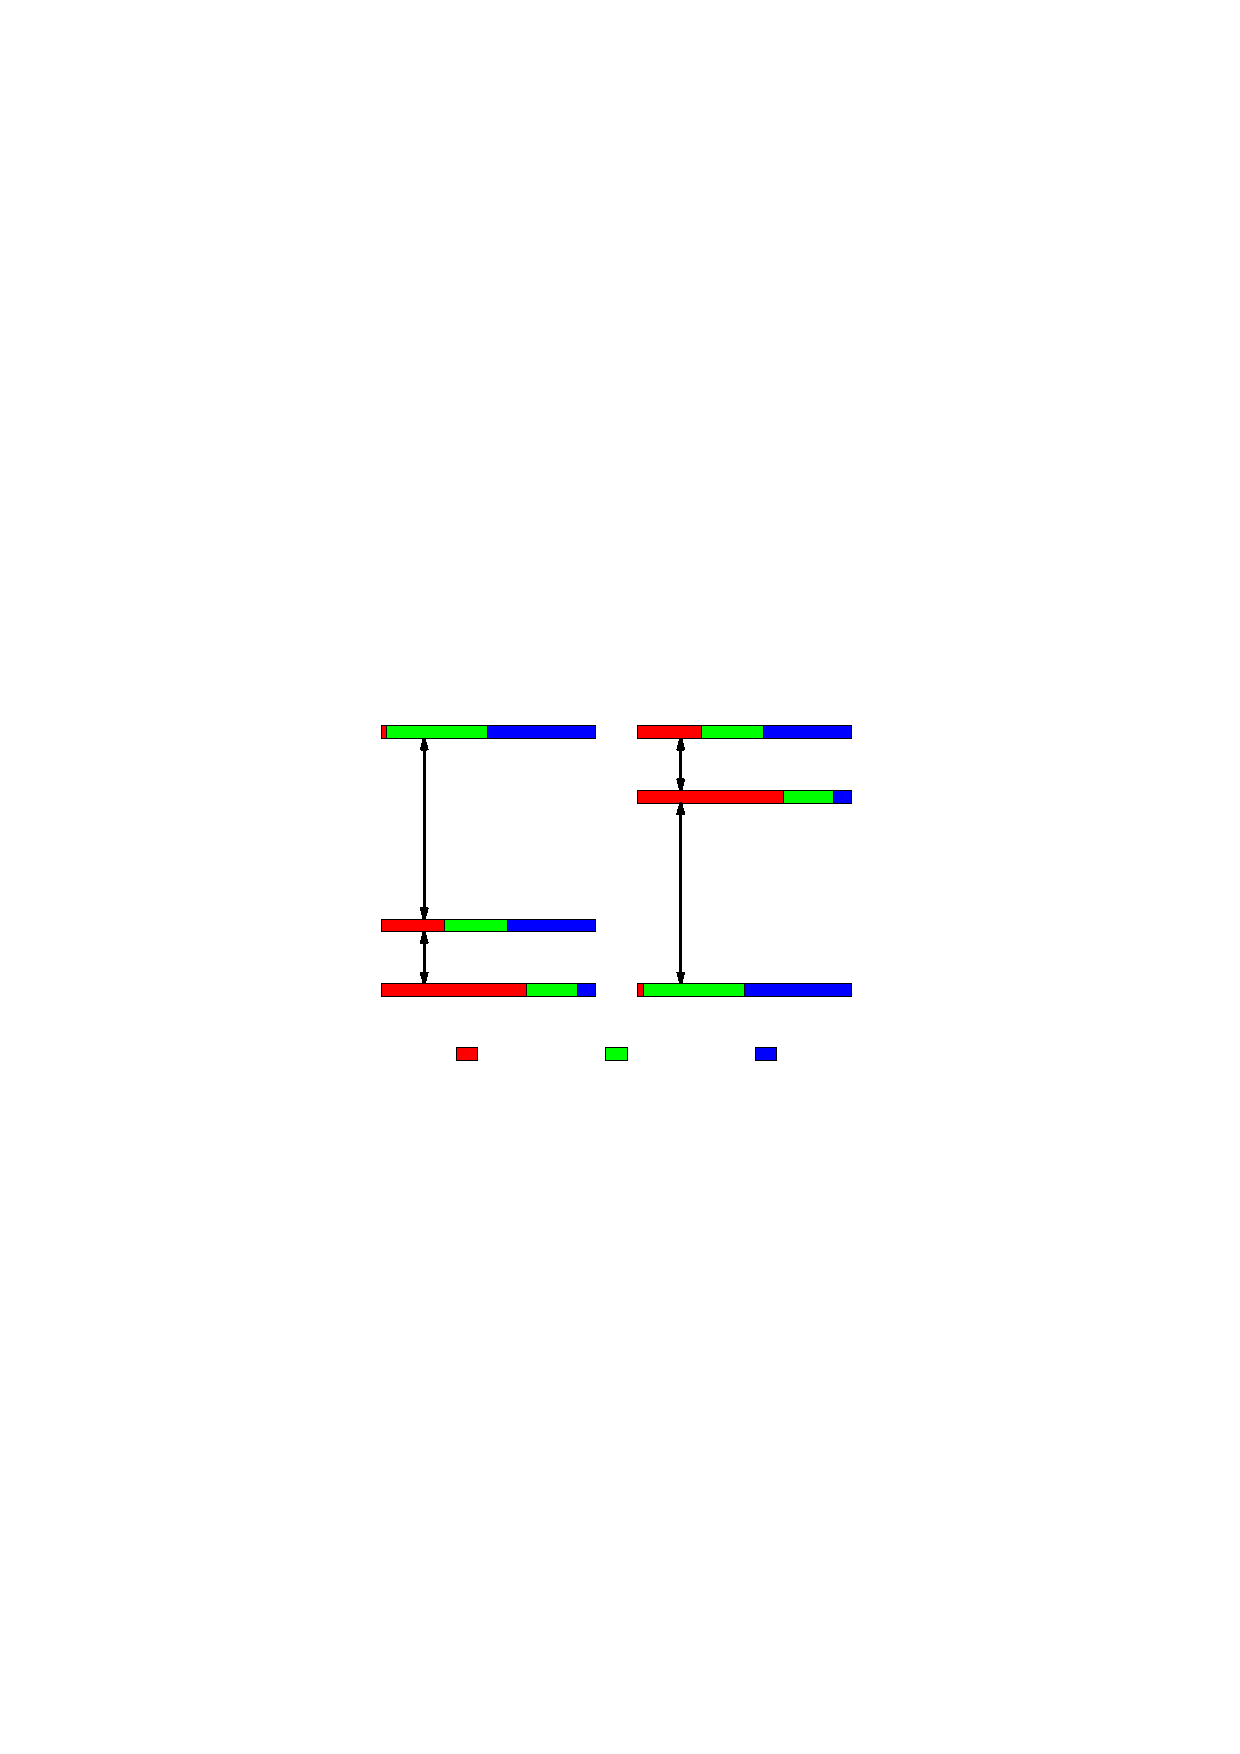
\includegraphics[scale=0.8]{img/h.pdf}
		\put(-170,145){Normal}
		\put(-75,145){Inverted}
		\put(-165,93){\footnotesize{$\Delta m^2_{31}$}}
		\put(-65,68){\footnotesize{$\Delta m^2_{31}$}}
		\put(-65,118){\footnotesize{$\Delta m^2_{21}$}}
		\put(-165,43){\footnotesize{$\Delta m^2_{21}$}}
		\put(-150,7){$\nu_e$}
		\put(-92,7){$\nu_\mu$}
		\put(-35,7){$\nu_\tau$}
		\put(-210,32){\footnotesize{$\nu_1$}}
		\put(-210,58){\footnotesize{$\nu_2$}}
		\put(-210,132){\footnotesize{$\nu_3$}}
		\put(-5,32){\footnotesize{$\nu_3$}}
		\put(-5,107){\footnotesize{$\nu_1$}}
		\put(-5,132){\footnotesize{$\nu_2$}}
		\caption{Neutrino mass hierarchy hypotheses.}\label{fig:ger}
	\end{figure}
%
		
		The JUNO experiment aims to measure the flux rate and energy spectrum of $\bar\nu_e\rightarrow\bar\nu_e$ oscillations to an unprecedentedly good degree of accuracy, especially to pin down the sign of $\Delta m^2_{31}$ or equivalently the neutrino mass ordering.
%
%		
	\subsection{The JUNO experiment}	%%%%%%%%%%%%%%%%%%%%%%%%%%%%%%%%%%%%%%%%%%%%%%%
%
%
		The Jiangmen Underground Neutrino Observatory (JUNO) is a multi-purpose neutrino experiment \cite{yellowbook}. It was proposed in 2008 to determine the neutrino mass hierarchy by detecting reactor antineutrinos from the Daya Bay nuclear power plant (NPP), thus formerly known as ``Daya Bay II experiment''. The mass hierarchy determination requires equal baselines from the detector to all reactor cores to avoid cancellation of the oscillation dephasing effect. Due to the complex and unclear layout of the future nuclear power plants in the neighborhood, the experiment was moved to Jiangmen city in Guangdong province in August 2012, and named as JUNO in 2013.
The site location is at 53 km from both the Yangjiang and Taishan NPPs. The JUNO project was approved by Chinese Academy of Sciences in February 2013. Data taking is expected in 2020.
		
		JUNO consists of a central detector, a water Cherenkov pool and a muon tracker. The central detector is a Liquid Scintillator (LS) detector of 20 kton fiducial mass with a designed energy resolution of $3\%/\sqrt{E/\mbox{MeV}}$. Both central detector (CD) and water pool (WP) are equipped with 20'' Photomultipliers Tubes (PMTs); they detect scintillation light in CD and Cherenkov light in WP.
		
		JUNO measures the reactor neutrino signal via the inverse beta decay reaction
%
		\begin{equation*}
			\bar\nu_e+p\rightarrow e^++n
		\end{equation*}
%
		in the LS. The reactor antineutrino $\bar\nu_e$ interacts with a proton, creating a positron ($e^+$) and a neutron. The positron quickly deposits its energy and annihilates into two 511-keV $\gamma$-rays, which gives a prompt signal. The neutron scatters in the detector until being thermalised. It is then captured by a proton, on average $200\mu s$ later, and releases a 2.2-MeV $\gamma$-ray. The coincidence of the prompt-delayed signal pair in such a short time significantly reduces backgrounds. The positron carries almost all energy of the neutrino in this reaction. All this can be visually represented as in Figure \ref{fig:detection}. The WP and an additional Top Tracker are used to measure muon tracks to reject cosmogenic backgrounds. Further details on JUNO physics can be found in \cite{yellowbook}.
%
		\begin{figure}[!h]
		\hspace{2 cm}
		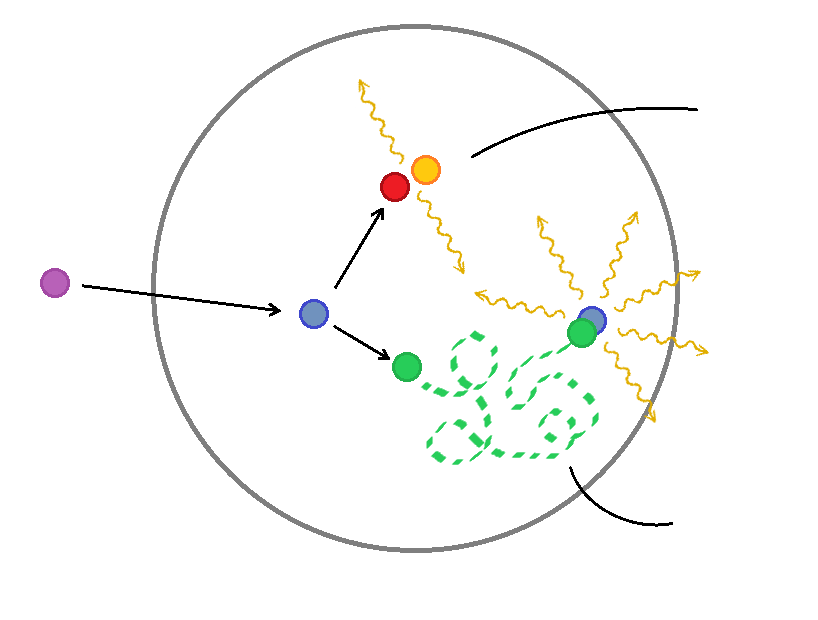
\includegraphics[scale=0.4]{img/gigidef.png}
		\put(-38,28){Thermalization}
		\put(-30,150){Prompt}
		\put(-25,80){Delayed}
		\put(-60,80){$p$}
		\put(-160,80){$p$}
		\put(-135,65){$n$}
		\put(-249,99){$\bar\nu_e$}
		\put(-142,132){$e^+$}
		\put(-123,143){$e^-$}
		\caption{Antineutrino detection in JUNO via inverse beta decay: the prompt signal is first detected, the delayed one comes, on average, after $200\mu$s.}\label{fig:detection}
		\end{figure}
%
%
	\section{Reactor antineutrino flux}	%%%%%%%%%%%%%%%%%%%%%%%%%%%%%%%%%%%%%%%%%%%%%%%
%
%		
		This section will focus on the evaluation of the number of electron antineutrinos $\bar{\nu}_e$ that would be detected at a far detector with medium baseline length from a reactor.
		
		In a nuclear reactor, antineutrinos are mainly produced via beta decay of the fission products of the four radio-active isotopes $^{235}$U, $^{238}$U, $^{239}$Pu and $^{241}$Pu in the fuel. The number of antineutrinos produced per fission depends on their energy $E_{\bar\nu_e}$ (MeV) \cite{ref4}
		\begin{equation*}
		\begin{split}
			\phi(E_{\bar\nu_e}) &= f_{^{235}\mathrm{U}}\; \exp(0.870-0.160E_{\bar\nu_e}-0.0910E^2_{\bar\nu_e}) \\
			&+ f_{^{239}\mathrm{Pu}} \exp(0.896-0.239E_{\bar\nu_e}-0.0981E^2_{\bar\nu_e}) \\
			&+ f_{^{238}\mathrm{U}}\:\: \exp(0.976-0.162E_{\bar\nu_e}-0.0790E^2_{\bar\nu_e}) \\
			&+ f_{^{241}\mathrm{Pu}} \exp(0.793-0.080E_{\bar\nu_e}-0.1085E^2_{\bar\nu_e}) \;,
		\end{split}
		\end{equation*}
		where $f_k$ denotes the relative fission contribution of the isotope $k$ in a reactor fuel, derived from the fission rate $N^\textup{fiss}_k$ of isotope $k$ as
		\begin{equation*}
			f_k:=\frac{N^\textup{fiss}_k}{\textstyle\sum_i N^\textup{fiss}_i}\;.
		\end{equation*}
		Although $f_k$ varies over time as the fuel is burned, it can be approximated for this type of experiments with the average value of the relative fission contributions: $f_{^{235}\mathrm{U}}=0.58$, $f_{^{239}\mathrm{Pu}}=0.30$, $f_{^{238}\mathrm{U}}=0.07$ and $f_{^{241}\mathrm{Pu}}=0.05$ \cite{ref5}. The event rate of antineutrinos with energy $E_{\bar\nu_e}$ (MeV) at a reactor of $P\;(\mbox{GW}_{\mbox{th}})$ thermal power is then expressed as
		\begin{equation}\label{eq:flux}
			\frac{dN}{dE_{\bar\nu_e}}=\frac{P}{\textstyle\sum_k f_k\epsilon_k}\phi(E_{\bar\nu_e})\cdot6.24\cdot10^{21}\;,
		\end{equation} 
		where $\epsilon_k$ is the released energy per fission of the isotope $k$: $\epsilon_{^{235}\mathrm{U}}=201.7$ MeV, $\epsilon_{^{239}\mathrm{Pu}}=210.0$ MeV, $\epsilon_{^{238}\mathrm{U}}=205.0$ MeV and $\epsilon_{^{234}\mathrm{Pu}}=212.4$ MeV \cite{ref6}. The numerical factor comes from unit conversion, 1GW/MeV $=6.24\cdot10^{21}$.
		
		This rate is then modulated by oscillation. The $\bar{\nu}_e$ survival probability (\ref{eq:pee}) is expressed as
		\begin{equation}\label{eq:pee2}
		\begin{split}
			P_{\bar\nu_e\rightarrow\bar\nu_e}\equiv P_{ee}=1 &- \cos^4\theta_{13}\sin^22\theta_{12}\sin^2\Delta_{21} \\
			&- \cos^2\theta_{12}\sin^22\theta_{13}\sin^2\Delta_{31} \\
			&- \sin^2\theta_{12}\sin^22\theta_{13}\sin^2\Delta_{32}\;,
		\end{split}
		\end{equation}
		The variables $m_i$ and $E_i$ are the mass and energy of the corresponding mass eigenstate, while $\theta_{ij}$ represent the neutrino mixing angles. The oscillation phases $\Delta_{ij}$ are defined as
		\begin{equation*}
			\Delta_{ij}:=\frac{\Delta m^2_{ij}L}{4E_{\bar\nu_e}}=1.27\cdot\frac{[\mbox{eV}^2][m]}{[\mbox{MeV}]}\;,\qquad(\Delta m^2_{ij}:=m_i^2-m_j^2)
		\end{equation*}
		with a baseline length from the reactor $L$.
		
		While $\Delta m_{21}^2$ is fixed, $\Delta m_{31}^2$ and then $\Delta m_{32}^2=\Delta m_{31}^2-\Delta m_{21}^2$ depend on the mass hierarchy:
		\begin{equation*}
			\Delta m_{31}^2=
			\begin{cases}
				\:m_3^2-m_1^2>0 \quad(\mbox{NH})\\
				\:m_3^2-m_1^2<0 \quad(\mbox{IH})
			\end{cases}.
		\end{equation*}
		As we have seen before JUNO uses protons as targets to detect electron antineutrinos via the inverse neutron beta decay (IBD) process
		\begin{equation*}
			\bar{\nu}_e+p\rightarrow e^++n\;.
		\end{equation*}
		The threshold neutrino energy of this process is $E_\textup{thr}\sim m_n-m_p+m_e\sim 1.804$ MeV, and the cross section is \cite{ref7}
		\begin{equation}\label{eq:sigma}
			\sigma_\textup{IBD}=E_{e^+}\:p_{e^+}\cdot9.52\cdot10^{-44}\;\mbox{cm}^2\;,
		\end{equation}
		where $E_{e^+}$ and $p_{e^+}$ are the energy and momentum of the positron in MeV, neglecting the kinetic energy of the proton and the neutron for a MeV scale antineutrino. The positron energy is roughly $E_{e^+}\sim E_{\bar\nu_e}-(m_n-m_p)$.
		
		The produced positron then interacts with scintillator, converting its kinetic energy to photons. Eventually, the positron annihilates with an electron in the detector and emits two 0.5 MeV photons. The energies of these photons are then accumulated as the visible energy $E_\textup{vis}$ which is the sum of the positron's total energy and the rest energy of one electron,
		\begin{equation*}
			E_\textup{vis}\sim E_{e^+}+m_e\sim(E_{\bar\nu_e}-0.78)\;\mbox{MeV}.
		\end{equation*}
		This shows that the antineutrino spectrum is simply shifted of 0.78 MeV circa from the visible spectrum.
		
		Finite detector energy resolution may distort the true visible energy $E_\textup{vis}$ to the finally observed one $E_\textup{vis}^\textup{obs}$. This effect can be modeled by a gaussian detector response function $G(E_\textup{vis}-E_\textup{vis}^\textup{obs},\delta E_\textup{vis})$ with the energy resolution $\delta E_\textup{vis}$
		\begin{equation}\label{eq:gauss}
			G(E_\textup{vis}-E_\textup{vis}^\textup{obs},\delta E_\textup{vis}) = \frac{1}{\sqrt{2\pi}\delta E_\textup{vis}} \exp\left\{-\frac{(E_\textup{vis}-E_\textup{vis}^\textup{obs})^2}{2(\delta E_\textup{vis})^2}\right\}.
		\end{equation}
		Generally the detector energy resolution can be modeled as
		\begin{equation}\label{eq:res}%
			\frac{\delta E_\textup{vis}}{E_\textup{vis}}=\sqrt{\frac{a^2}{E_\textup{vis}}+b^2}
		\end{equation}%
%		
		\begin{figure}[t]
			%\centering
			\begin{tikzpicture}
				\begin{semilogxaxis}[xmin=1,xmax=7,ymin=0,ymax=1000,
								xlabel=$E_\textup{vis}^\textup{obs}$ (MeV),
								ylabel=$\frac{dN}{dE_\textup{vis}^\textup{obs}}$, ylabel style={rotate=-90},
								width=11cm, height=6cm,
								legend style={draw=none},
								log ticks with fixed point,
								xtick=\empty,
                                 					extra x ticks={2,...,10},
                                 					extra x tick labels={2,...,10}]
								
					\addplot [thick,blue]
					file {data/curveIdealNH.txt};
					\addplot [dash pattern=on 5pt off 1pt, thick,red]
					file {data/curveIdealIH.txt};
					\legend {NH, IH}

				\end{semilogxaxis}
			\end{tikzpicture}
			\caption{Energy spectrum for $10^5$ events, infinite resolution, assuming normal (blue) or inverted (dashed red) hierarchy. It's clear how the $\sin^22\theta_{13}$ is responsible for the high frequency oscillation while $\sin^22\theta_{12}$ is responsible for the lowest one.}\label{fig:ideal}
		\end{figure}%
%		
		($E_\textup{vis}$ in MeV) and is composed of two parts. The first term in the square-root represents the statistical uncertainty, and the second one gives the sistematic uncertainty, which will not be considered in this study. The observed antineutrino distribution by a detector with $N_p$ free protons after an exposure time $T$ can then be expressed, from (\ref{eq:flux}), (\ref{eq:pee2}), (\ref{eq:sigma}) and (\ref{eq:gauss}), as
		\begin{equation}\label{eq:spectrum}%
			\frac{dN}{dE_\textup{vis}^\textup{obs}}=\frac{N_pT}{4\pi L^2}\int_{E_\textup{thr}}^\infty dE_{\bar\nu_e}\frac{dN}{dE_{\bar\nu_e}}P_{ee}(L,E_{\bar\nu_e})\:\sigma_\textup{IBD}(E_{\bar\nu_e})\:G(E_{\bar\nu_e}-0.78-E_\textup{vis}^\textup{obs},\delta E_\textup{vis}^\textup{obs}).
		\end{equation}
		The energy spectrum measured by JUNO assuming infinite and finite energy resolution is given in Figures \ref{fig:ideal} and \ref{fig:res}, respectively.
%		
		%oppure meglio cos�
		%\begin{equation}\label{eq:spectrum}%
		%\begin{split}
			%\frac{dN}{dE_\textup{vis}^\textup{obs}}&=\frac{N_pT}{4\pi L^2}\int_{E_\textup{thr}}^\infty dE_{\bar\nu_e}\frac{dN}{dE_{\bar\nu_e}}P_{ee}(L,E_{\bar\nu_e}) \\
			%&\cdot\sigma_\textup{IBD}(E_{\bar\nu_e})G(E_{\bar\nu_e}-0.8-E_\textup{vis}^\textup{obs},\delta E_\textup{vis}).
		%\end{split}
		%\end{equation}
%
		\begin{figure}[!b]
			%\centering
			\begin{tikzpicture}
				\begin{semilogxaxis}[xmin=1,xmax=7,ymin=0,ymax=1000,
								xlabel=$E_\textup{vis}^\textup{obs}$ (MeV),
								ylabel=$\frac{dN}{dE_\textup{vis}^\textup{obs}}$, ylabel style={rotate=-90},
								width=11cm, height=6cm,
								legend style={draw=none},
								log ticks with fixed point,
								xtick=\empty,
                                 					extra x ticks={2,...,10},
                                 					extra x tick labels={2,...,10}]
								
					\addplot [thick,blue]
					file {data/curveNH.txt};
					\addplot [dash pattern=on 5pt off 1pt,thick,red]
					file {data/curveIH.txt};
					\legend {NH, IH}

				\end{semilogxaxis}
			\end{tikzpicture}
			\caption{Energy spectrum assuming $10^5$ events, $a=3\%$, and normal (blue) or inverted (dashed red) hierarchy.}\label{fig:res}
		\end{figure}
%
%
	\section{Sensitivity to the mass hierarchy}	%%%%%%%%%%%%%%%%%%%%%%%%%%%%%%%%%%%%%%%%%%%
%
%	
		After obtaining the energy distribution of reactor antineutrinos, a further step concerns the estimation of the sensitivity in determining the mass hierarchy using a $\chi^2$ analysis. To set the stage, we introduce the $\chi^2$ function as
		\begin{equation}\label{eq:chi}
		\chi^2=\chi^2_\textup{stat}+\chi^2_\textup{para}\;.
		\end{equation}
		The first term represents the statistical fluctuation, when binning w.r.t. $E_\textup{vis}^\textup{obs}$ is introduced it looks like
		\begin{equation*}
			\chi^2_\textup{stat}=\sum_i \left(\frac{N_i-N_i^*}{\sqrt{N_i^*}}\right)^2\;,
		\end{equation*}
		with the summation running over all the bins. Here $N_i^*$ is the number of events for the $i_{th}$ bin while $N_i$ is the theoretical prediction assuming right or wrong mass hierarchy.
		
		The second term summarizes the prior knowledge on mixing parameters. In JUNO these are the mixing angles $\sin^22\theta_{12}$ and $\sin^22\theta_{13}$, and the two mass-square differences, $\Delta m^2_{21}$ and $\Delta m_{31}^2$ (the latter with the sign depending on the mass hierarchy assumption), whose contributions look like
		\begin{equation*}
		\begin{split}
			\chi^2_\textup{para} &= \left(\frac{\sin^22\theta_{12}-(\sin^22\theta_{12})_\textup{input}}{\delta \sin^22\theta_{12}}\right)^2 \\
			&+ \left(\frac{\sin^22\theta_{13}-(\sin^22\theta_{13})_\textup{input}}{\delta \sin^22\theta_{13}}\right)^2 \\
			&+ \left(\frac{\Delta m^2_{21}-(\Delta m^2_{21})_\textup{input}}{\delta \Delta m^2_{21}}\right)^2 \\
			&+ \left(\frac{\Delta m^2_{31}-(\Delta m^2_{31})_\textup{input}}{\delta \Delta m^2_{31}}\right)^2\;.
		\end{split}
		\end{equation*}		
		
		We then define $\Delta\chi^2$ as
		\begin{equation*}
			\Delta\chi^2:=\chi^2_\textup{wrong}-\chi^2_\textup{true}\;,
		\end{equation*}
		where $\chi^2_\textup{wrong}$ is the minimum of the $\chi^2$ calculated assuming the wrong hierarchy and $\chi^2_\textup{true}$ is the minimum of the $\chi^2$ calculated assuming the correct hierarchy. It will eventually be scaled with the number of degrees of freedom, which is clearly equal to the number of fitted data minus the constraints: $n_\textup{bin}-6$.
%		
%
%
%
	\section{Data simulation and fitting}	%%%%%%%%%%%%%%%%%%%%%%%%%%%%%%%%%%%%%%%%%%%%%%%
%
%
		All the datasets used in this study are simulated within the ROOT Data Analysis Framework \cite{root}, mainly using the built-in Monte Carlo method \texttt{TF1::GetRandom} to take into account statistical fluctuations. They are all composed of $10^5$ events, which is a realistic assumption considering that the expected event rate calculated with the JUNO experimental setup is around 60 events/day\footnote{With two reactors of 36 GW thermal power at 53 km, a 20-kton Liquid Scintillator detector.} \cite{yellowbook} for a total running time of 5 years. The values of the two mixing angles and the two mass-square differences used in the generation are listed in Table 1.
%
		\begin{table}[!h]
		\centering
		\caption{The input values $Y^\textup{input}$ and their uncertainties $\delta Y$ taken from \cite{ref8,ref9,ref10}.}
			\begin{tabular}{ccccc}
				\toprule
				Y	&	$\sin^22\theta_{12}$	&	$\sin^22\theta_{13}$	&	$\Delta m^2_{21}\:\mbox{eV}^2$	&	$|\Delta m^2_{31}|\:\mbox{eV}^2$	\\
				\midrule
				$Y^\textup{input}$	&	0.857	&	0.089	&	$7.50\times10^{-5}$	&	$2.32\times10^{-3}$	\\
				$\delta Y$			&	0.024	&	0.005	&	$0.20\times10^{-5}$	&	$0.11\times10^{-3}$	\\
				\bottomrule
			\end{tabular}
		\end{table}
%

		To take into account the finite detector resolution (\ref{eq:res}) an alternative generation method has been chosen. The adoption of the method presented above for the infinite resolution case implies knowing the explicit analytic form (without the integral) of the spectrum function, which is fundamentally impossible to find, cfr. eq. (\ref{eq:spectrum}). This study proceeded as follows: random events ($E^\textup{true}_i$ being their energies) were generated following the ideal distribution ($a=0$); then, before filling the histogram, assigned to a new energy value following the normal gaussian distribution with mean $E^\textup{true}_i$ and variance $a\sqrt{E^\textup{true}_i}$. This is a highly efficient way to generate datasets with finite resolution.
		
		The minimisation of (\ref{eq:chi}) required the direct use of the ROOT minimisation libraries in the fitting procedure, in particular the \texttt{TMinuit} algorithm\footnote{See the appendix.}. Throughout the minimisation procedure all the parameters were left free to vary in their physical limits, except for the baseline length, which was fixed, assuming a very small error $\delta L$ on it.
%
%
%
	\section{Results}			%%%%%%%%%%%%%%%%%%%%%%%%%%%%%%%%%%%%%%%%%%%%%%%
%
%		
	\subsection{Infinite resolution: sensitivity and baseline length}	%%%%%%%%%%%%%%%%%%%%%%%%%%%%%%%%%%%%%%%%%%%%%%%
%
%
		\begin{figure}[b]
		\centering
			\centerline{
			\begin{minipage}[c]{.60\textwidth}
				\centering
				\captionsetup{justification=centering,margin=0cm}
				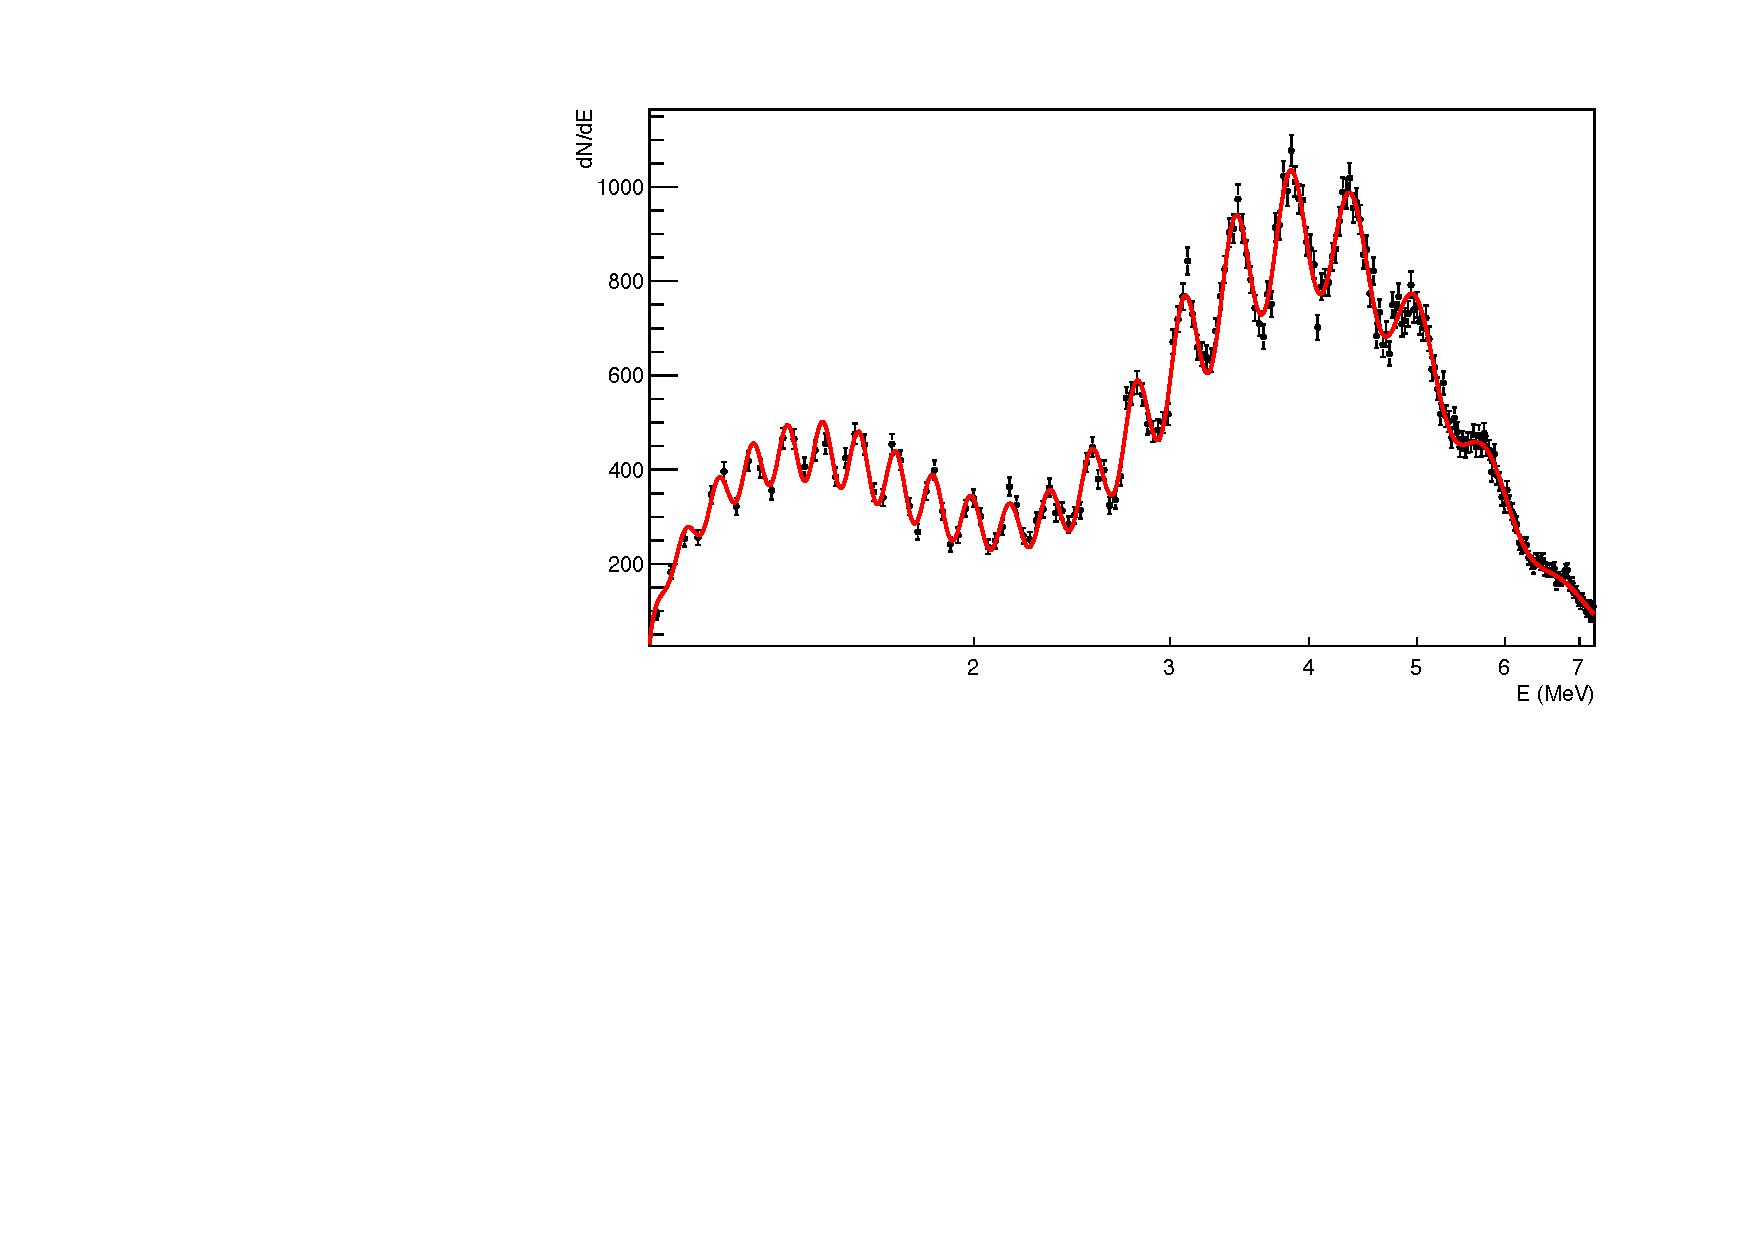
\includegraphics[scale=0.4]{img/plotMinuitIdealNH50.pdf}
				\caption{Fitting NH data with NH \\ theory at $L=50$ km.}\label{fig:50kmNH}
			\end{minipage}%
			\hspace{-1cm}
			\begin{minipage}[c]{.60\textwidth}
				\centering
				\captionsetup{justification=centering,margin=0cm}
				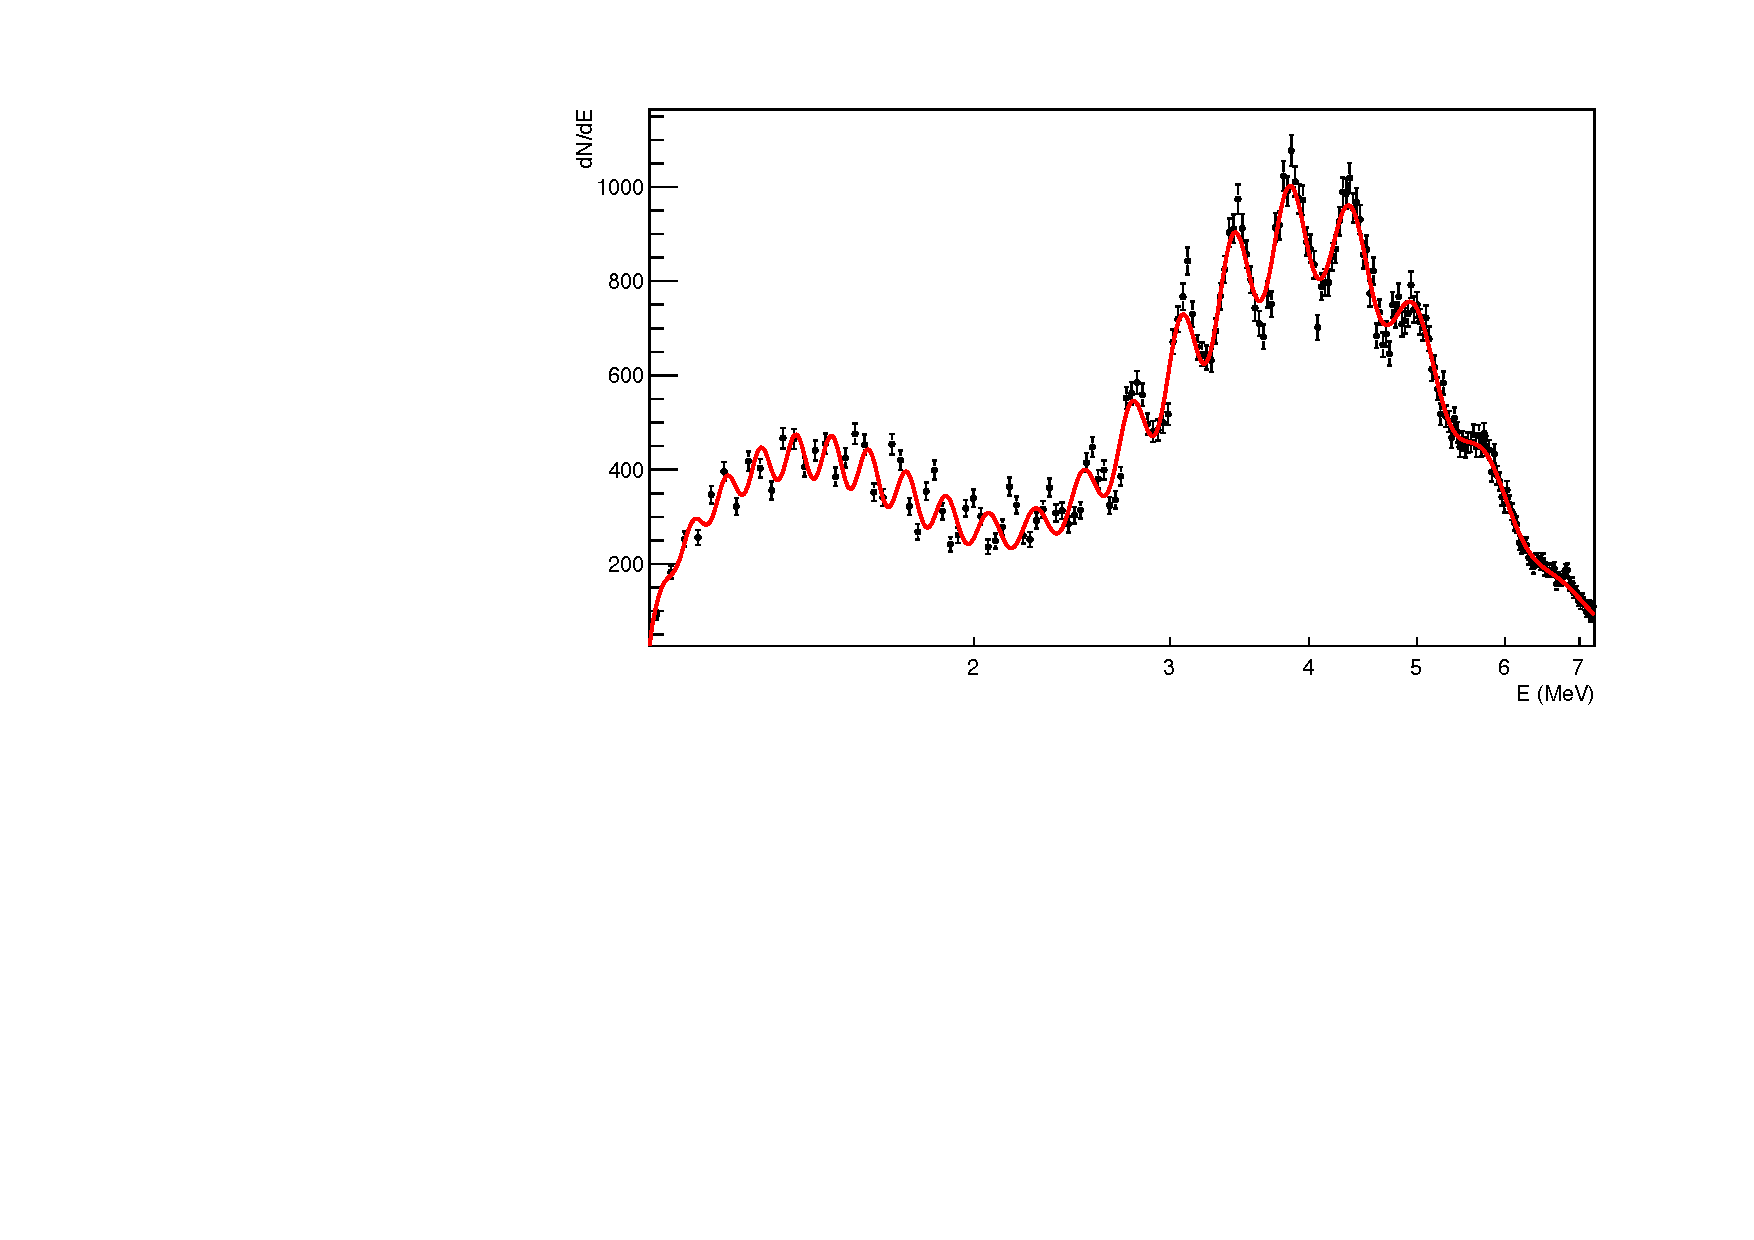
\includegraphics[scale=0.4]{img/plotMinuitIdealIH50.pdf}
				\caption{Fitting NH data with IH \\ theory at $L=50$ km.}\label{fig:50kmIH}
			\end{minipage}
			}
		\end{figure}
%
		This section will discuss the results obtained assuming infinite resolution ($a=0$). The number of bins can be arbitrary high in this case, so 200 bins were chosen as unit. We present the study of the baseline length influence on the sensitivity in distinguishing between the two theoretical hypotheses, namely between normal and inverted hierarchy. 
		
		Two different setups, at $L=50$ km and $L=30$ km, have been considered and a fit on NH data, assuming normal or inverted mass hierarchy, has been performed. A preliminary look at the results at 50 km presented in Figures \ref{fig:50kmNH} and \ref{fig:50kmIH}, shows that the parameter that changes the most at the end of the minimisation procedure is $\sin^22\theta_{13}$, which is responsible for the tiny oscillations; Furthermore the total lack of adherence to data in the first 2 MeV it's self-evident. The difference between the two $\chi^2_\textup{min}$ values, $\Delta\chi^2$, is a powerful statistic test to discriminate between normal and inverted hierarchy. In this specific case we find $\Delta\chi^2/ndf\sim0.6$.
		
		On the other side, comparing results at 30 km in Figures \ref{fig:70kmNH} and \ref{fig:70kmIH} it can be noticed how it's harder to establish which fit is the ``wrong'' one. That's because both theoretical hypotheses seem to fit data accurately, as a matter of fact we find $\Delta\chi^2/ndf\sim0$. As a consequence the sensitivity in discriminating between the two theories is higher in the first case and we can say for sure that it strongly depends on the baseline length $L$.
%		
		\begin{figure}[t]
			\centerline{
			\begin{minipage}[c]{.60\textwidth}
				\centering
				\captionsetup{justification=centering,margin=0cm}
				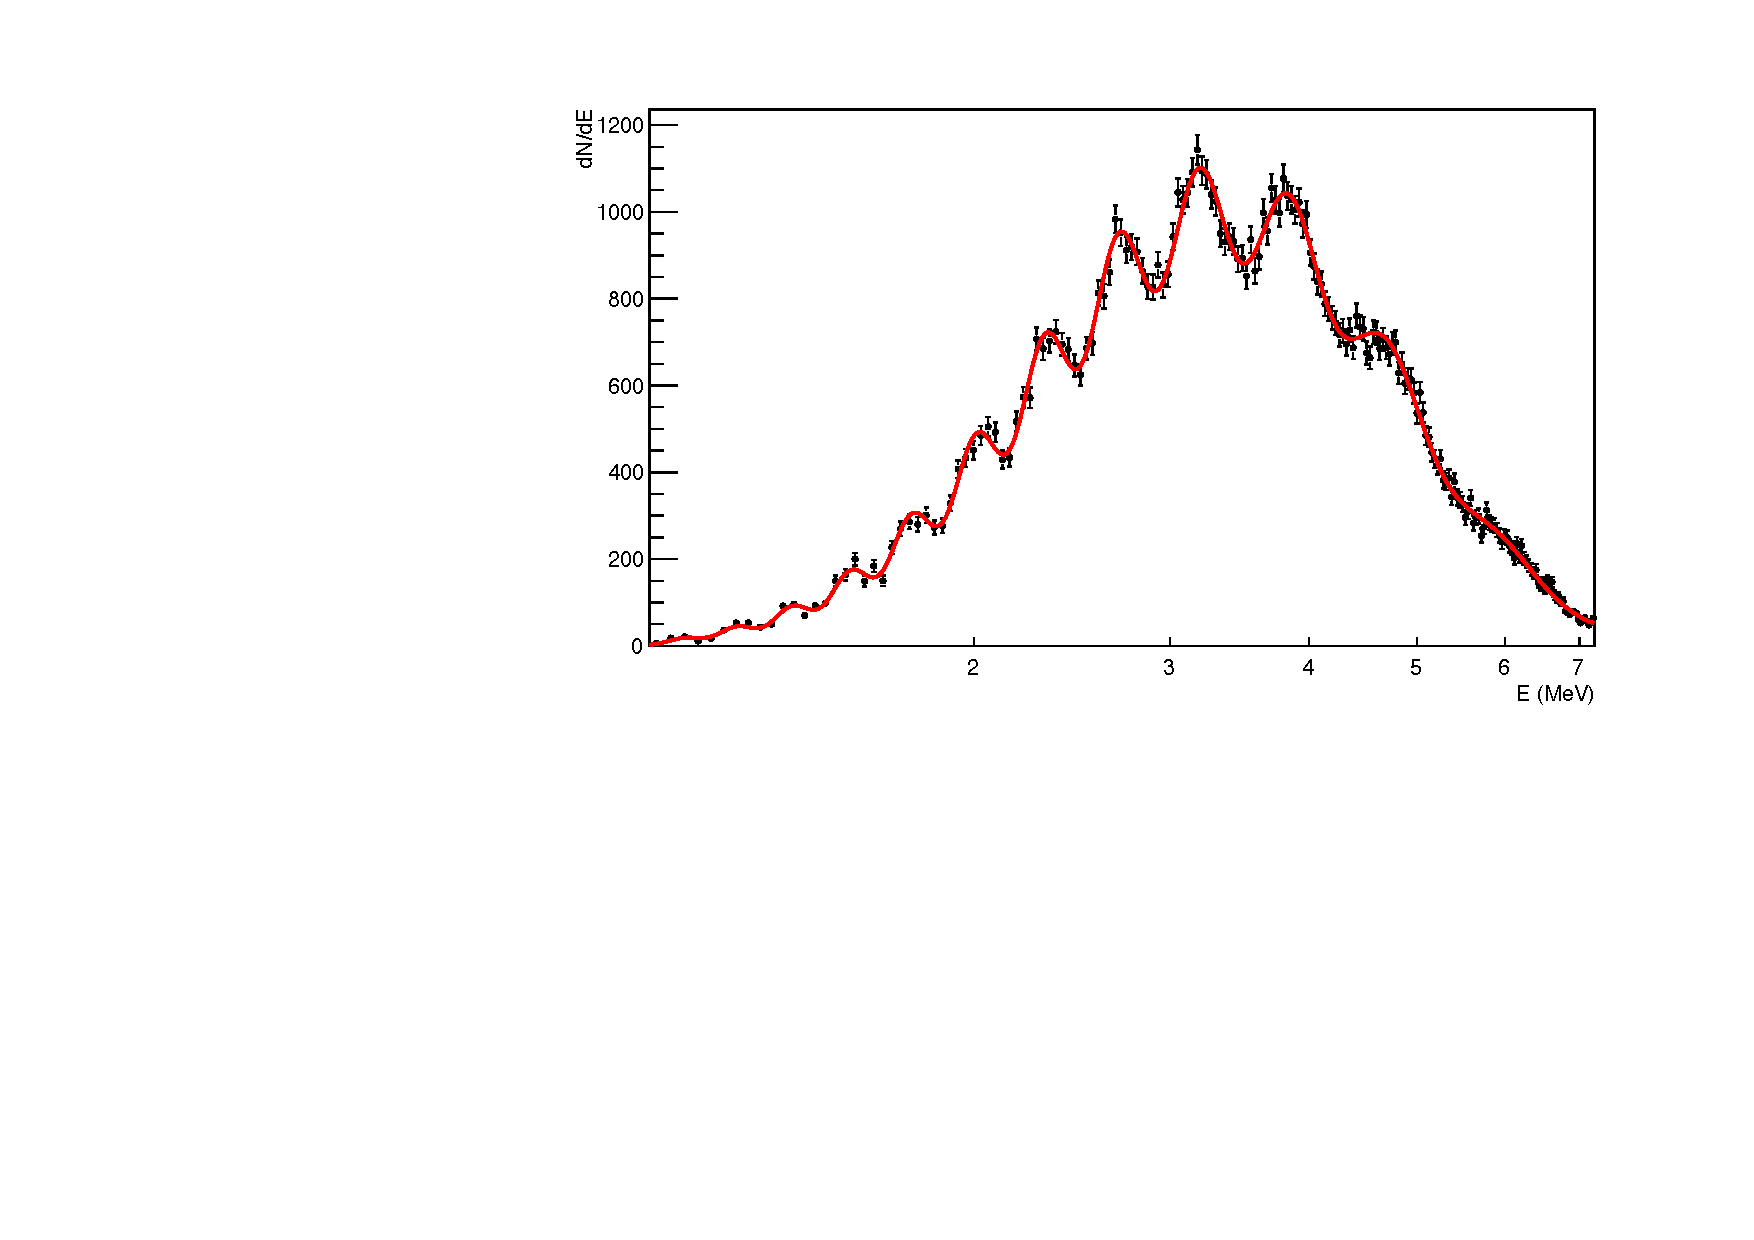
\includegraphics[scale=0.4]{img/plotMinuitIdealNH30.pdf}
				\caption{Fitting NH data with NH \\ theory at $L=30$ km.}\label{fig:70kmNH}
			\end{minipage}%
			\hspace{-1cm}
			\begin{minipage}[c]{.60\textwidth}
				\centering
				\captionsetup{justification=centering,margin=0cm}
				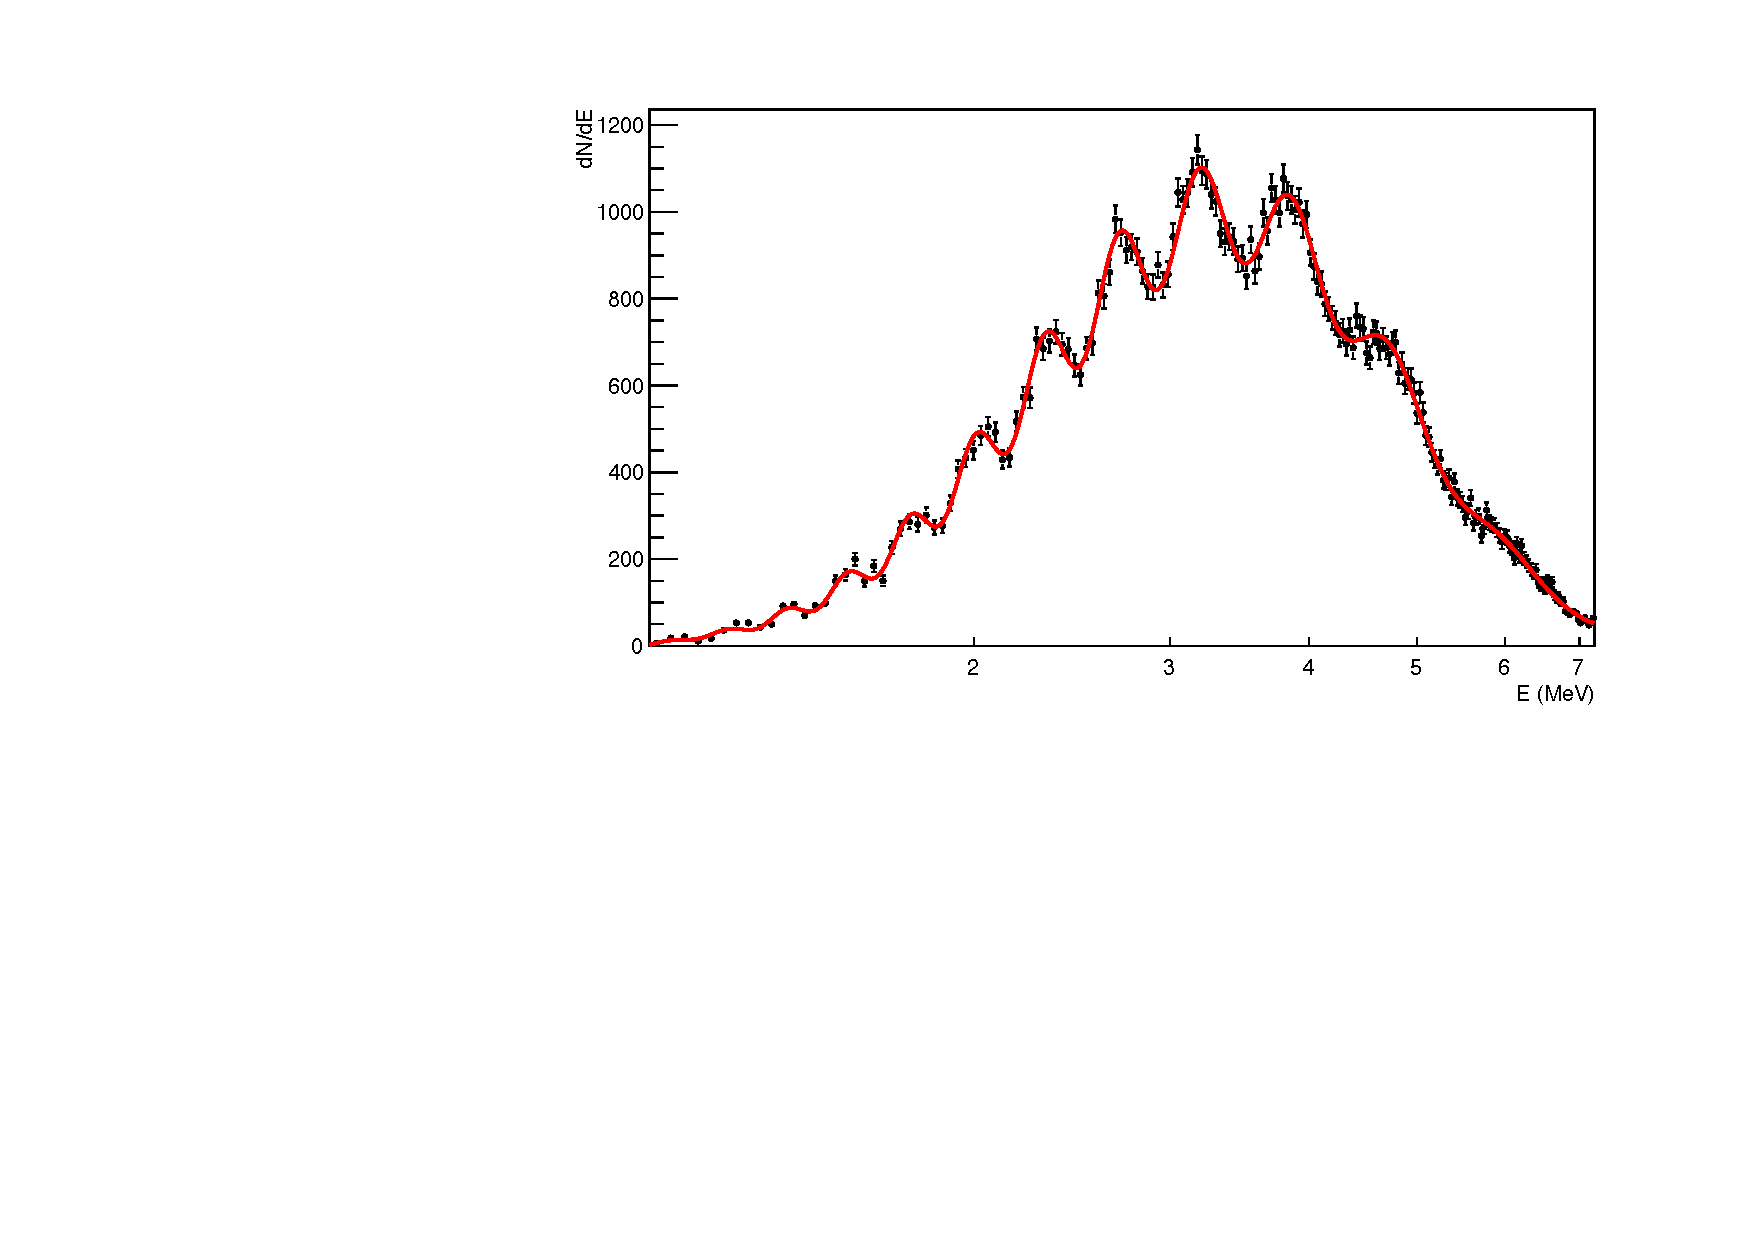
\includegraphics[scale=0.4]{img/plotMinuitIdealIH30.pdf}
				\caption{Fitting NH data with IH \\ theory at $L=30$ km.}\label{fig:70kmIH}
			\end{minipage}
			}
		\end{figure}
%
		\begin{figure}[!b]
			\centering
			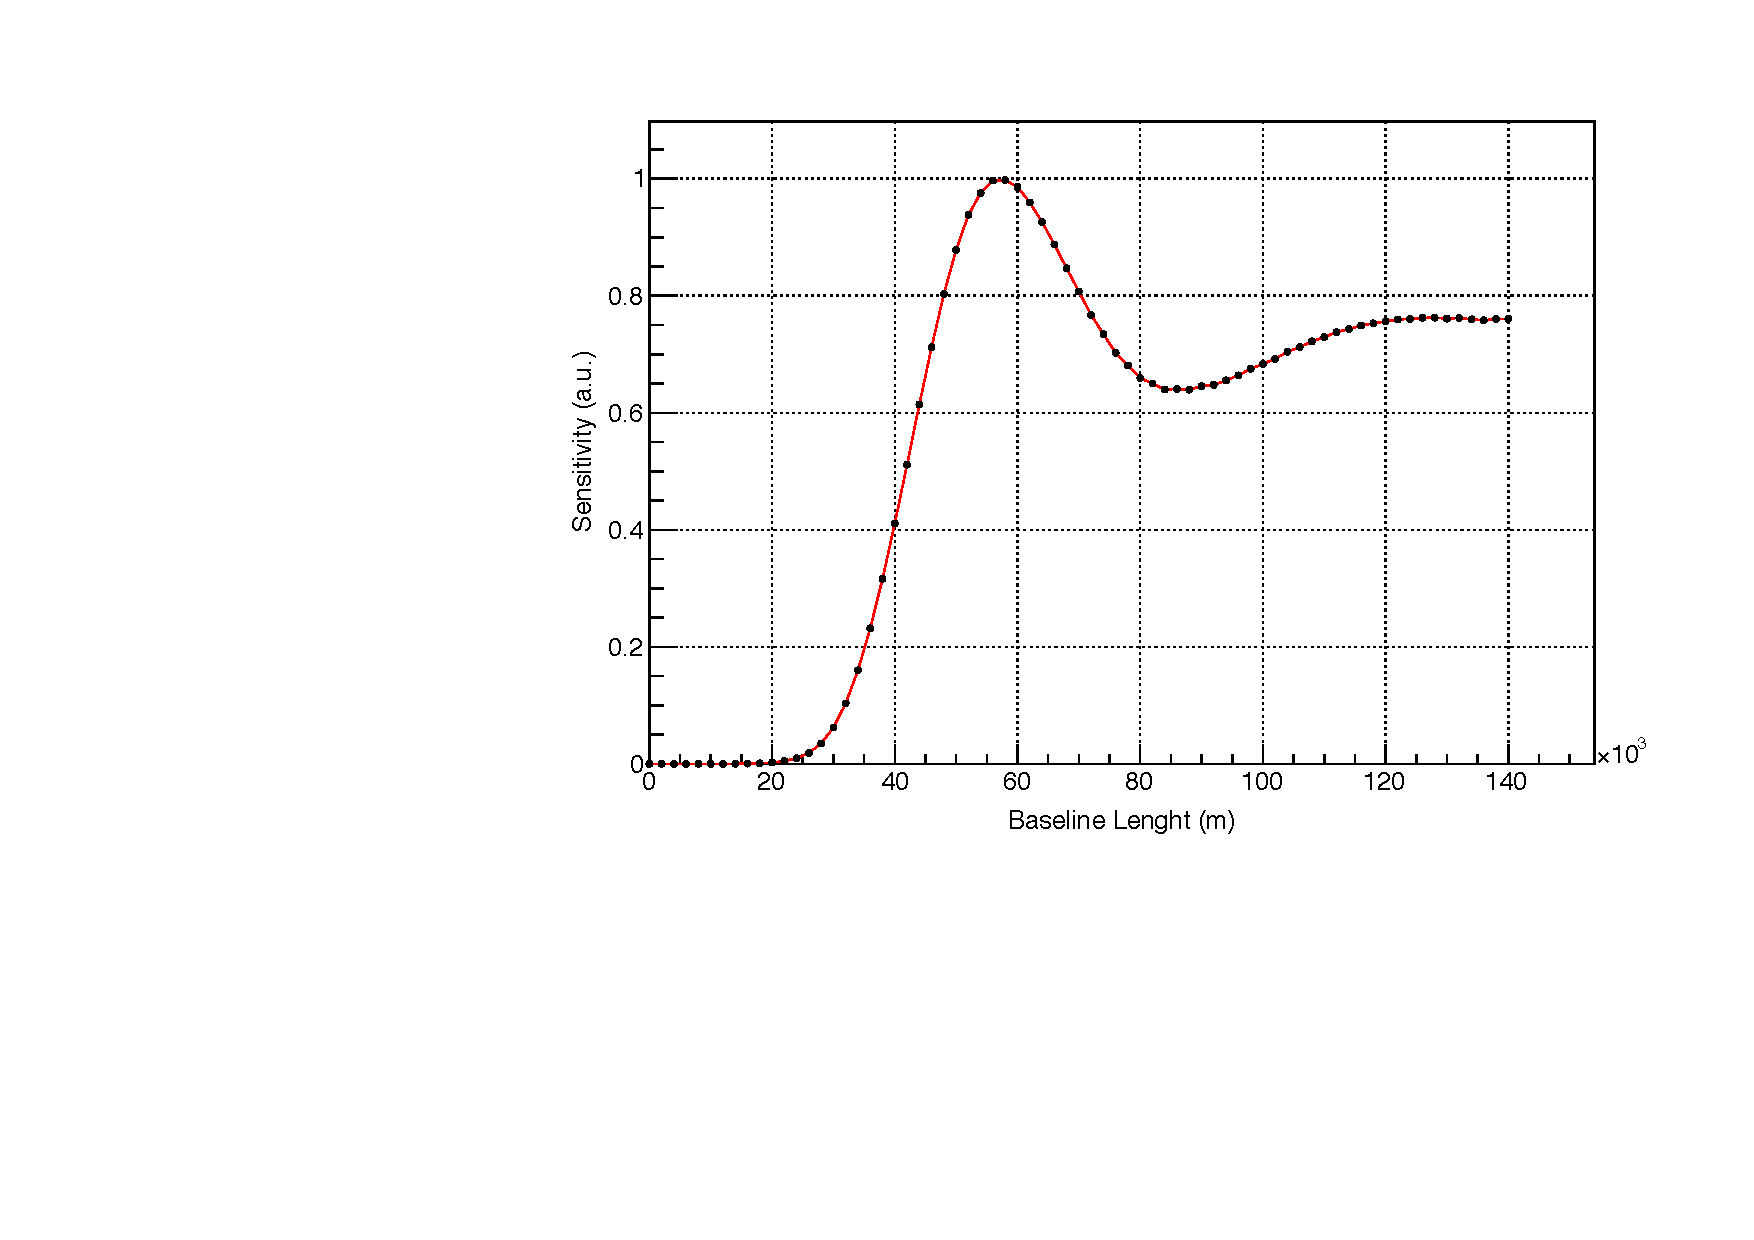
\includegraphics[scale=0.46]{img/chi2baseline_new.pdf}
			\caption{Sensitivity in arbitrary units ($\Delta\chi^2$ normalized to 1 at the peak) w.r.t. the baseline length, assuming $a=0$.}\label{fig:baseline}
		\end{figure}
%

		Distances from 1 to 140 km between the detector and the reactor cores, $L$, were considered in the calculation of $\Delta\chi^2$. It has been chosen to fit Asimov datasets \cite{asimov} (where the bin's content is equal to the expectation value) with 400 bins to avoid useless fluctuations in the plot. The results presented in Figure \ref{fig:baseline} clearly show that a range exists, from 50 km to 70 km, with a maximum in $\sim55$ km, in which the sensitivity is maximised, allowing to better discriminate between the two hypotheses. One may look for a second, higher, maximum for $L>140$ km, but since antineutrino rate (see \ref{eq:spectrum}) is proportional to $1/L^2$, the time spent collecting the same amount of data would be prohibitive.
		
		As the next section will explain, the study of the sensitivity w.r.t. the baseline length with finite resolution has not been performed, due to a high computational time request. In \cite{giappi} this analysis shows how the peak's position moves toward smaller values of $L$ increasing the $a$ value in (\ref{eq:res}).
%
%
	\subsection{Finite resolution: sensitivity and resolution}	%%%%%%%%%%%%%%%%%%%%%%%%%%%%%%%%%%%%%%%%%%%%%%%%%%%
%
%
\begin{figure}[!t]
	\centering
	\begin{tikzpicture}
	\begin{groupplot}[
 		group style={group name=my plots,
        				    group size=1 by 3,
        				    xlabels at=edge bottom,
        				    xticklabels at=edge bottom,
        				    vertical sep=0pt},
   		width=11cm,
    		height=3cm,
    		xlabel=$E$ (MeV),
    		ylabel style={rotate=-90},
    		log ticks with fixed point,
    		xmin=1, xmax=7,
    		ymin=0, ymax=1150,
		ytick=\empty,
		xtick=\empty]
%		
		\nextgroupplot[xmode=log]
			\addplot [thick, blue] file {data/curveNH2.txt};
			\addplot [dash pattern=on 5pt off 1pt,thick, red]   file {data/curveIH2.txt};
%
		\nextgroupplot[xmode=log,
				       ylabel=$\frac{dN}{dE}$]
%
			\addplot [thick,blue] file {data/curveNH4.txt};
			\addplot [dash pattern=on 5pt off 1pt,thick,red]   file {data/curveIH4.txt};
%
		\nextgroupplot[xmode=log,
   				       extra x ticks={1,2,...,10},
    				       extra x tick labels={1,2,...,10},
    				       xtick pos=left,]
%				       
			\addplot [thick,blue] file {data/curveNH6.txt};
			\addplot [dash pattern=on 5pt off 1pt,thick,red]   file {data/curveIH6.txt};
%
	\end{groupplot}
	\end{tikzpicture}
	\put(-270,140){\footnotesize{$a=2\%$}}
	\put(-270,100){\footnotesize{$a=4\%$}}
	\put(-270,60){\footnotesize{$a=6\%$}}
	\caption{Plots of the spectrum \ref{eq:spectrum} with $a=$ 2\%, 4\%, 6\% resolution.}\label{fig:diffres}
\end{figure}
%		
		\begin{figure}[!b]
			\centerline{
			\begin{minipage}[c]{.60\textwidth}
				\centering
				\captionsetup{justification=centering,margin=0cm}
				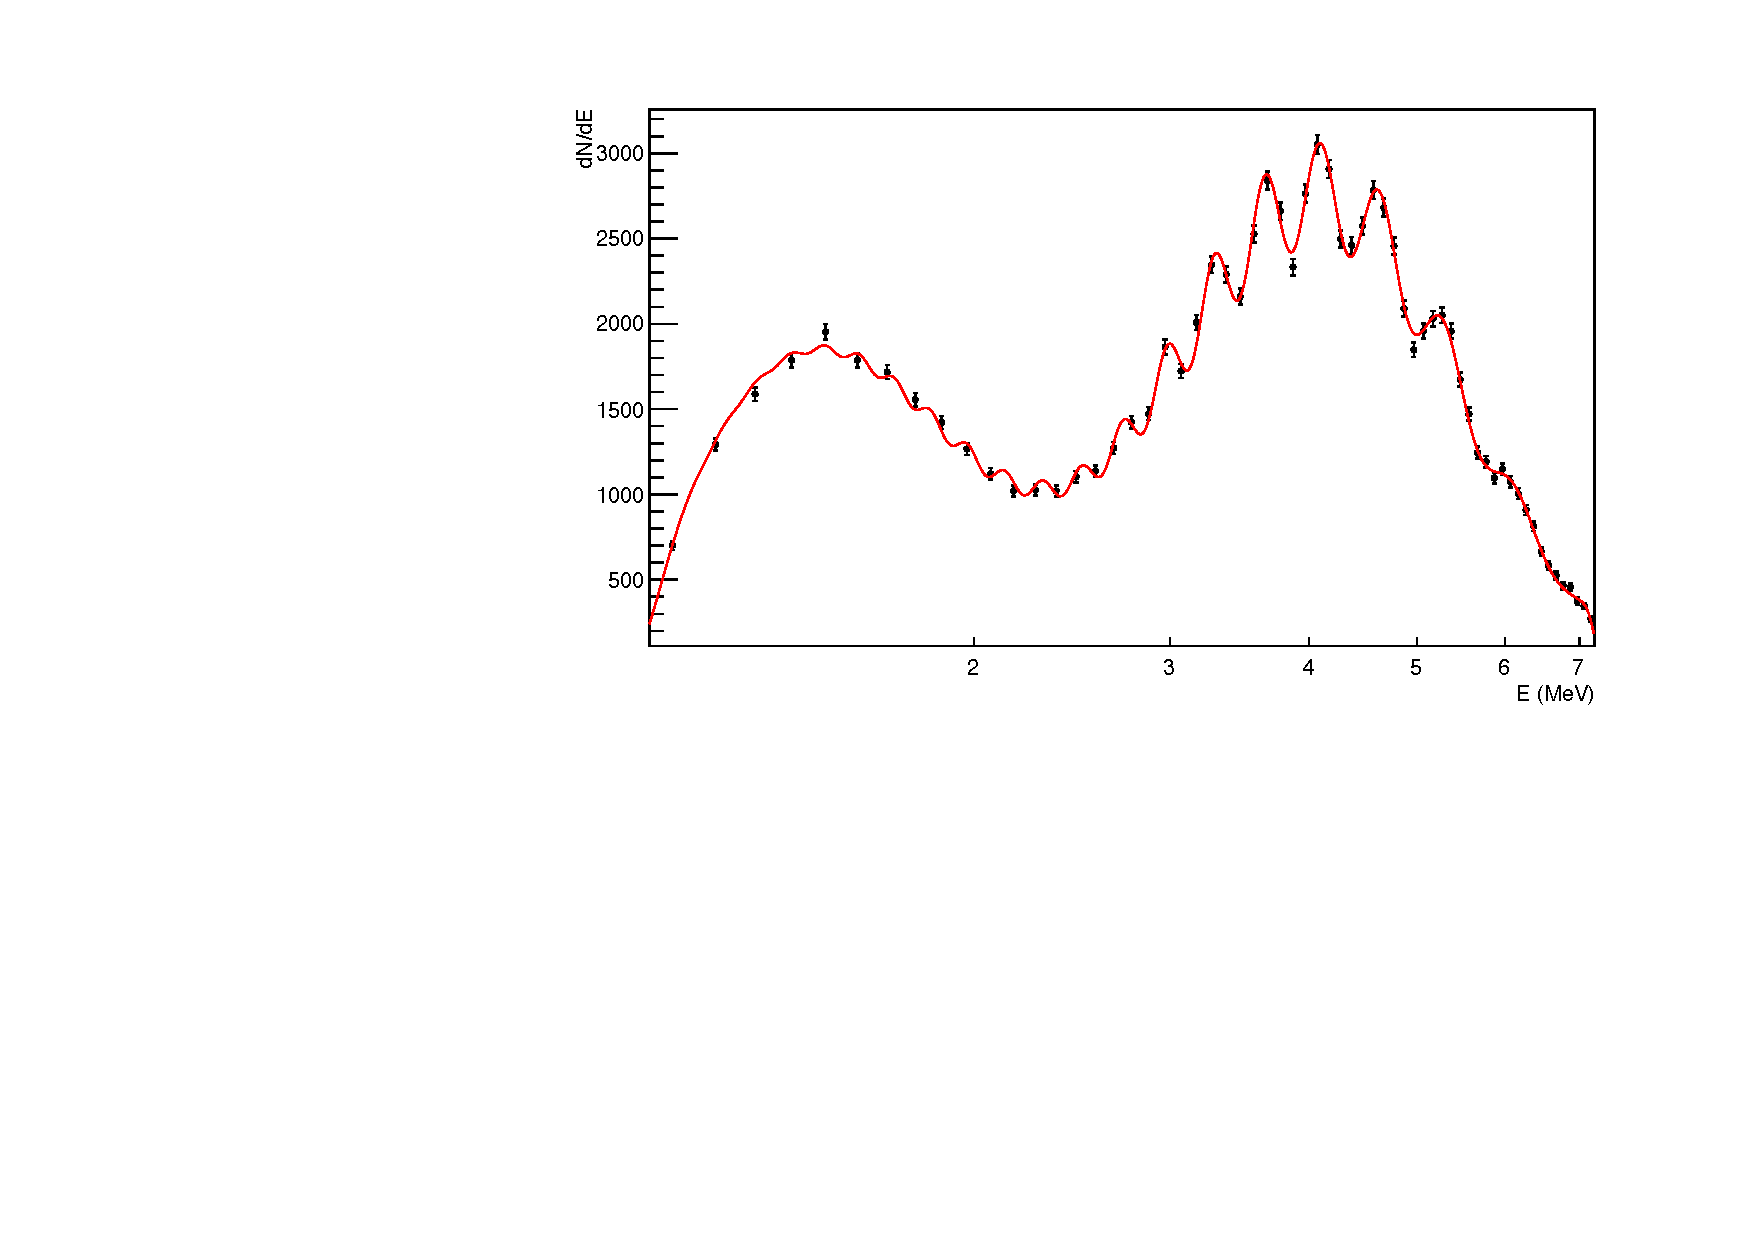
\includegraphics[scale=0.4]{img/plotMinuitResNH3.pdf}
				\caption{Fitting NH data with NH \\theory, $a=3\%$ at $L=53$ km.}\label{fig:resfitNH}
			\end{minipage}%
			\hspace{-1cm}
			\begin{minipage}[c]{.60\textwidth}
				\centering
				\captionsetup{justification=centering,margin=0cm}
				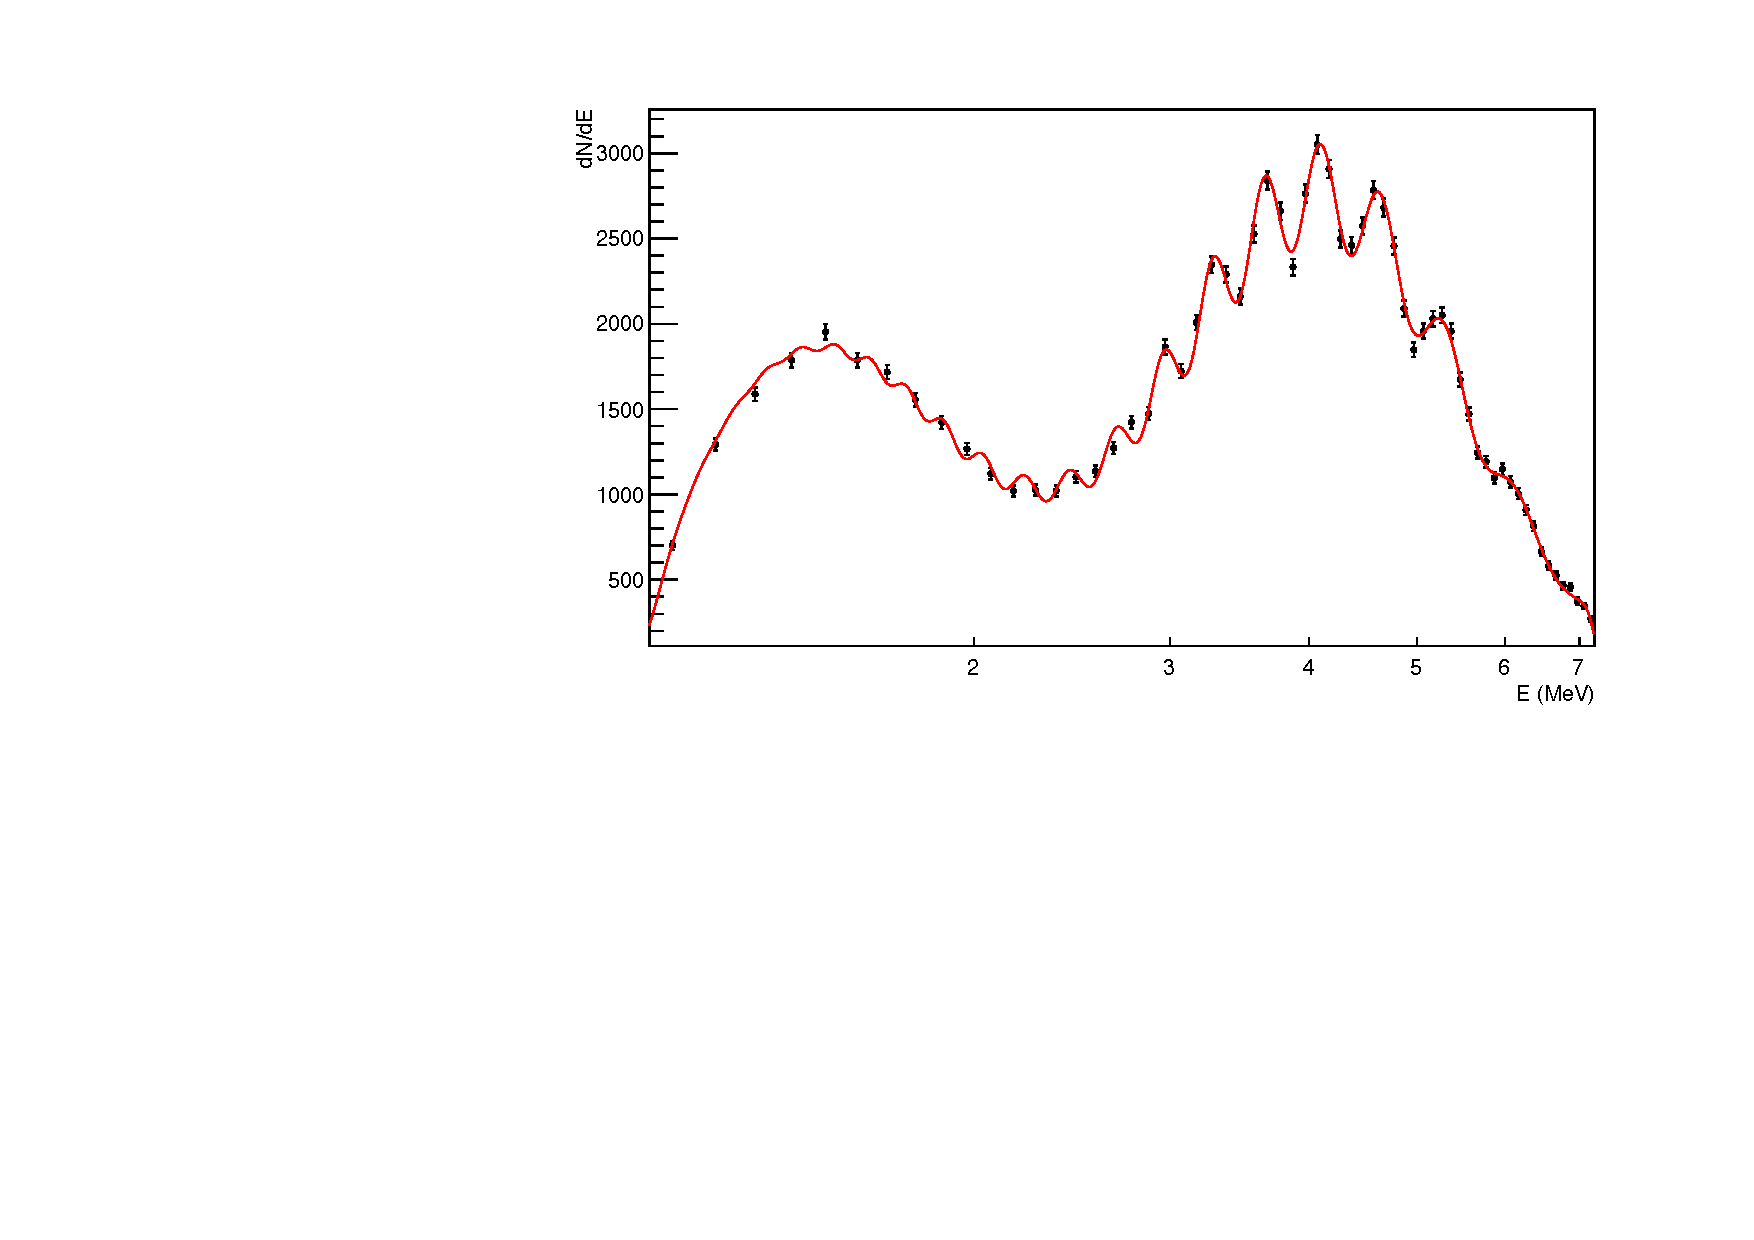
\includegraphics[scale=0.4]{img/plotMinuitResIH3.pdf}
				\caption{Fitting NH data with IH \\theory, $a=3\%$ at $L=53$ km.}\label{fig:resfitIH}
			\end{minipage}
			}
		\end{figure}
%

		Introducing a finite resolution in the fitting process is not trivial\footnote{Details of the chosen programming method in the appendix.}, as seen before the problem involves the presence of an integral in the expression (\ref{eq:spectrum}). Sensitivity will now be examined by comparing spectrums collected at the same baseline length (at 53 km, as planned) but with different values of the experimental resolution. As it can be seen with just an overlook to the three graphs in Figure \ref{fig:diffres}, the difference between the two curves (normal and inverted hierarchy) vanishes when decreasing the resolution parameter, from a (experimentally challenging) $2\%/\sqrt{E/\mbox{MeV}}$ resolution to a much worse $6\%/\sqrt{E/\mbox{MeV}}$. The resolution effect is particularly strong in the first part, between 0 and 2 MeV, where the tiny oscillations are totally smeared out and the curves are nearly indistinguishable.

		Let's now consider the binning issue. Choosing an arbitrarily high number of bins makes little sense with a finite resolution, a realistic binning of 100 keV was therefore adopted, which signifies more or less 62 bins through the entire spectrum.
		
		We discuss as a preliminary analysis the results of fitting NH data (resolution 3\%/$\sqrt{E/\mbox{MeV}}$) either with correct or wrong theory (Figures \ref{fig:resfitNH} and \ref{fig:resfitIH}). As can be seen, comparing this with Figures \ref{fig:50kmNH} and \ref{fig:50kmIH}, now it's very hard to say which fit is the ``wrong'' one, as the bins are less than in the ideal case and the two datasets almost superimposable. This means that the two $\chi^2$ are very similar and the $\Delta\chi^2$ is therefore very small. 
%
	\begin{figure}[!t]
		\centering
		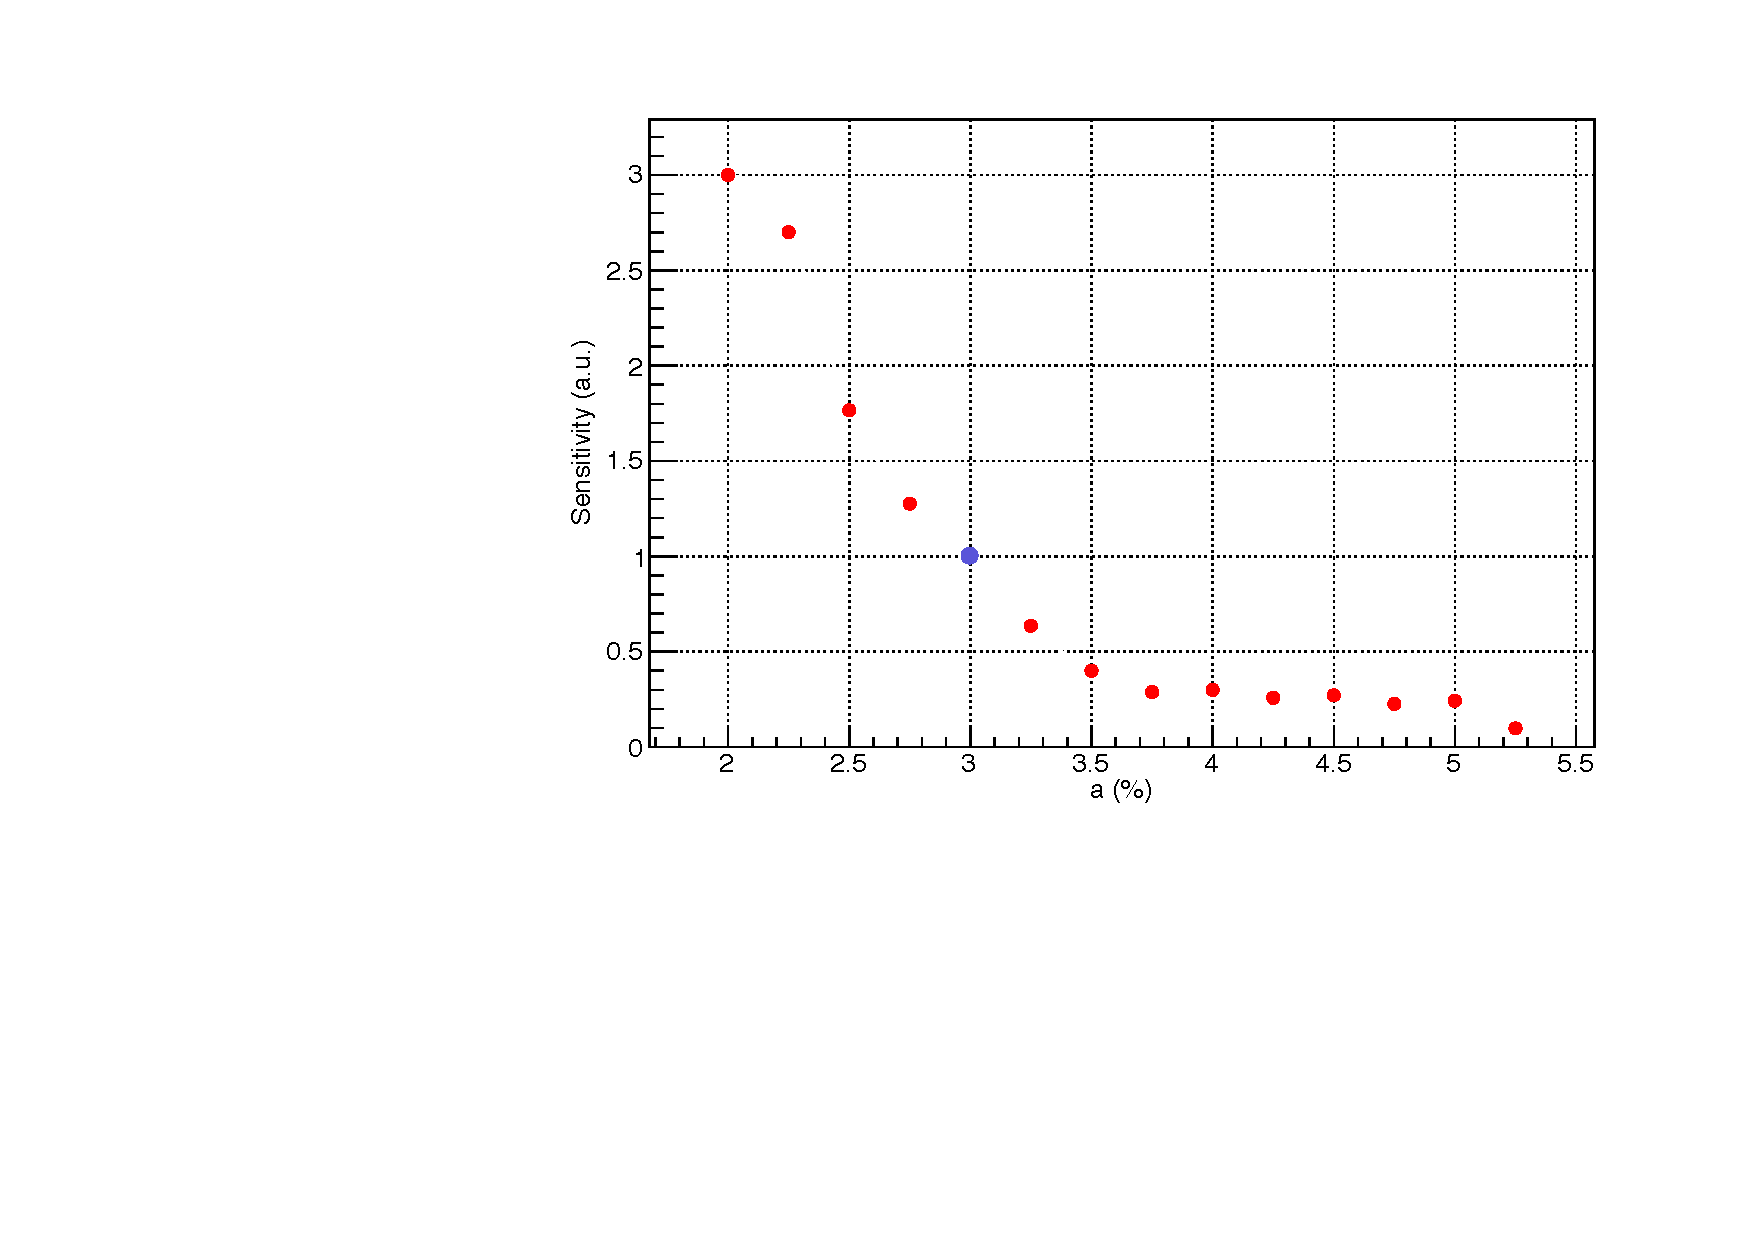
\includegraphics[scale=0.5]{img/sensres_new2.pdf}
		\caption{Sensitivity in arbitrary units ($\Delta\chi^2$ normalized to 1 at 3\% resolution) w.r.t. the statistical factor $a$ in the resolution expression at $L=53$ km.}\label{fig:sensres}
	\end{figure}
%
		
		Because of the complexity of the expression (\ref{eq:spectrum}), performing this kind of minimisation with the available processors requires a non-negligible amount of computational time. This drawback is a significant limit in the kind of analysis this section focuses on; a plot with the same number of points as the one in Figure \ref{fig:baseline} is, computationally speaking, too expensive. In addition to this, with $a<2\%$ the ROOT algorithm fails to compute the integral with the standard level of tolerance, and setting a higher level would obviously be more time-consuming. With regards to studying the sensitivity ($\Delta\chi^2$) w.r.t. the resolution parameter $a$ we can only make a qualitative analysis.
		
		Finally, let's examine the graph in Figure \ref{fig:sensres}. Each of the fourteen points is the result of the mean of three different values of $\Delta\chi^2$, computed considering three datasets simulated with the same set of parameters but with a different seed in the generation of the random events. This cuts out the effects of the statistical fluctuations on $\chi^2$ and any bad-precision issues in the minimisation algorithm. The $\Delta\chi^2$ results are normalized to make the sensitivity at the JUNO designed resolution $3\%/\sqrt{E/\mbox{MeV}}$ unitary. It is straightforward to notice that sensitivity rapidly goes to zero when the resolution worsens, in particular with $a>3\%$ the ability to discriminate between the two hypotheses is practically zero. We can easily conclude that any resolution equal or better than the designed one is essential to determinate the mass hierarchy with an acceptable accuracy.
%		
	\section{Discussion and conclusions}	%%%%%%%%%%%%%%%%%%%%%%%%%%%%%%%%%%%%%%%%%%%%%%%
%	
%	
		The sensitivity of the JUNO experiment to the determination of the neutrino mass hierarchy has been studied by performing a $\chi^2$ analysis. The results are applicable to all medium baseline reactor electron-antineutrino oscillation experiments with scintillation detection system and a simular active mass.
		
		Taking into account statistical fluctuations in the data and finite bin-size effects, we study the impacts of the baseline length and the energy resolution on the sensitivity, represented by the $\Delta\chi^2$, and find that it strongly depends on them. With infinite resolution ($a=0$) the optimal baseline length is found to be in the interval $[50,70]$ km and at the actual indicated JUNO site ($L=53$ km) an energy resolution better or equal to the 3\%/$\sqrt{E/\mbox{MeV}}$ level is needed to determine the neutrino mass hierarchy pattern. With these experimental settings, JUNO would be able to determine the mass hierarchy after no less five years of running.
%
%
	\section*{Acknowledgments}
%
		We wish to thank Prof.~Fabio Mantovani, Prof.~Vito Antonelli, Dott.~Marica Baldoncini and all the members of the JUNO Italy MC Group. They had an essential role in the first organization phase of this research work; we got essential support in understanding the JUNO physics and, last but not least, a warm hospitality at the JUNO Monte Carlo Workshop held in July at the Department of Physics and Earth Sciences of the Ferrara University. We also would like to thank Prof.~Riccardo Brugnera for all the further valuable discussions.
%
%
%
%
%
%
%
\appendix
\setcounter{secnumdepth}{0}
\definecolor{dkgreen}{rgb}{0,0.6,0}
\definecolor{gray}{rgb}{0.5,0.5,0.5}
\definecolor{mauve}{rgb}{0.58,0,0.82}

\lstset{%frame=tb,
  language=c++,
  aboveskip=3mm,
  belowskip=3mm,
  showstringspaces=false,
  columns=flexible,
  basicstyle={\small\ttfamily},
  numbers=none,
  numberstyle=\tiny\color{gray},
  keywordstyle=\color{blue},
  commentstyle=\color{dkgreen},
  stringstyle=\color{mauve},
  breaklines=true,
  breakatwhitespace=true,
  tabsize=3
}

\section[Appendix]{Appendix: Fitting with the \texttt{TMinuit} class}
	When performing a fit not only minimising the standard $\chi^2$
	\[
		\chi^2_\textup{std}=\sum_i \left(\frac{N_i-N_i^*}{\sqrt{N_i^*}}\right)^2
	\]
	but a more general function (referred to as $\chi^2$ for the remainder of this section), the build-in ROOT method \texttt{TF1::Fit} is no longer exploitable. Given data and a \texttt{TF1} object, this method uses the \texttt{TMinuit} libraries in order to minimise $\chi^2_\textup{std}$ and efficiently provide results. Is therefore necessary to explicitly write the chosen $\chi^2$ function and directly use \texttt{TMinuit} to minimise it.
	
	Let's first consider the infinite resolution case of the spectrum (\ref{eq:spectrum}), when its expression it's explicit. After declaring the \texttt{TMinuit} object that performs the minimisation (\texttt{gMinuit}), the function that needs minimising (\texttt{myFCN}), that is to say the $\chi^2$ function, must be set with the command
	\begin{lstlisting}
	gMinuit->SetFCN(myFCN);
	\end{lstlisting}
	The implementation of \texttt{myFCN} must be standard \cite{root}:
	\begin{lstlisting}
	void myFCN( int &npar, double* gin, double &f, double* par, int flag) {
		f = ... ;	// implement the function
	}
	\end{lstlisting}
	where \texttt{f} is the value of the $\chi^2$ function, \texttt{par} is the pointer to the array of function parameters and \texttt{npar} its dimension; \texttt{TMinuit} will vary the values it points in the minimisation procedure. The other arguments will not be considered for the purpose of this section. In the specific case we are examining, we can calculate the value of the $\chi^2_\textup{std}$ using a \texttt{for} loop:
	\begin{lstlisting}
	double chi2 = 0;
	double* xi = new double[1];
	for ( int i = 1 ; i <= dataset->GetSize()-2 ; ++i ) {
	
		xi[0] = Emin + (Emax-Emin)/(2*N_div) + (i-1)*(Emax-Emin)/N_div;	
			// bin's mid point
		chi2 += pow( (spectrum->EvalPar( xi , par ) - dataset->GetBinContent(i)) / datasetNH->GetBinError(i) ,2);
	}
	f = chi2;
	\end{lstlisting}
	where \texttt{spectrum} is a \texttt{TF1} object corresponding to our theoretical distribution with its parameters and \texttt{dataset} is a \texttt{TH1F} object with \texttt{N\_div} number of bins between the range $[\texttt{Emin},\texttt{Emax}]$ containing the data to fit. Is important to note that \texttt{spectrum} is evaluated in each bin's mid point and in the parameter values pointed toby \texttt{par}, the latter being passed from the \texttt{TMinuit} object to \texttt{myFCN} to test the $\chi^2$ value during the minimisation procedure. This implementation allows the user to change the $\chi^2_\textup{std}$ expression or add other terms. 
	
	Now that the function to minimise is set we can initialise the parameters and add their limits with the \texttt{mnparm} function, then launch the minimisation procedure with the \texttt{mnexcm} function. There are three algorithms in \texttt{TMinuit}: \texttt{SEEK} consists in a preliminary Monte Carlo search of the minimum, \texttt{SIMPLEX} quickly finds its rough value and \texttt{MIGRAD} improves the estimation. \texttt{SEEK} it's often used to find the absolute minimum before improving it, as a matter of fact it can happen that \texttt{SIMPLEX} or \texttt{MIGRAD} converges to a minimum which is only local.
	
	Applying this procedure to the finite resolution case calls for further code enhancement to bypass the absence of an explicit form of the spectrum as above, therefore using a \texttt{TF1} object to represent it is now obviously impossible. The sleight of hand required to overcome this obstacle is writing the integrand of (\ref{eq:spectrum}) 
	\begin{equation*}
		f(E,\hat{E})=\frac{N_pT}{4\pi L^2}\frac{dN}{dE}(E)\:P_{ee}(E)\:\sigma_\textup{IBD}(E)\:G(E-0.78-\hat{E},\delta \hat{E})
	\end{equation*}
	as a \texttt{TF1} with $E$ as the main variable $x$ and $\hat{E}$ as a parameter, then when calculating $\chi^2$ integrating in $dE$ for every point using $\hat{E}$ as the main variable. The code is presented below:
	\begin{lstlisting}
	for ( int i = 1 ; i <= dataset->GetSize()-2 ; ++i ) {
	
		par[7] = Emin + (Emax-Emin)/(2*N_div_R) + (i-1)*(Emax-Emin)/N_div_R;
		chi2 += pow( ( integrand->Integral( Ethr , Max , par , 1E-13) - dataset->GetBinContent(i)) / dataset->GetBinError(i) ,2);
   	}
	\end{lstlisting}
	The parameter \texttt{par[7]} represents $\hat{E}$, \texttt{Ethr} it's the energy threshold, \texttt{Max} a sufficient high energy value where the antineutrino distribution is practically zero, and the fourth argument of \texttt{TF1::Integral} is the tolerance set in the ROOT's integration algorithm. The parameters value must also be called back from the \texttt{TMinuit} object before every calculation of $\chi^2$ inserting
	\begin{lstlisting}
	for ( int i = 0 ; i < npar ; ++i ) {
		gMinuit->GetParameter( i , par[i] , parErr[i] );
		}	
	\end{lstlisting}
	inside the \texttt{myFCN} declaration before the \texttt{for} loop.
	
	Unlike the first version, which requires negligible computational time in this kind of analysis, this code it's definitely time-consuming: a complete minimisation takes several minutes. This is due to the calculation of the integral, which is not trivial even with numerical methods; decreasing the tolerance value obviously creates additional processing time.
	
	The limits given by the complex kind of integration also influence the range of resolution values we want to test. For $a<2\%$ the integration algorithm with a tolerance of $10^{-13}$ hardly converges all over the points, and the value of $\chi^2$ is then distorted. A smaller tolerance value would clearly prevents this issue, but the amount of required time for each iteration becomes unacceptable when the need to iterate it in a program that acts in a large number of situations arises.	

%
%
%
%
%
%
	\clearpage
	\addcontentsline{toc}{section}{\refname}
	\begin{thebibliography}{9}
%
		\bibitem{bettini}
		A.~Bettini, \emph{Introduction to elementary Particle Physics}, Cambridge University Press, 2014.
%
		\bibitem{weinberg}
		S.~Weinberg, \emph{A Model of Leptons, Phys.~Rev.~Lett.} 19 (1967) 1264
%
		\bibitem{davis}
		R.~Davis, D.~S.~Harmer and K.~C.~Hoffman,\emph{A Search for Neutrinos from the Sun, Phys.~Rev.~Lett.} 20 (1968) 1205.
%
		\bibitem{bahcall}
		J.~N.~Bachall and C.~Pena-Garay, \emph{Solar Models and Solar Neutrino Oscillations}, New J.~Phys. 6 (2004) 63.
%
		\bibitem{MNS}
		Z.~Maki, M.~Nakagawa, S.~Sakata, \emph{Remarks on the Unified Model of Elementary Particles,
Progr.~Theor.~Phys.} 28 (1962) 870.
%
		\bibitem{P}
		B.~Pontecorvo, \emph{Inverse beta processes and nonconservation of lepton charge,
Sov.~Phys.~JETP} 7 (1958) 172.
%
		\bibitem{rif1}
		Z.~z.~Xing and S ~Zhou, \emph{Neutrinos in particle physics, astronomy and cosmology}, Springer-Verlag, Berlin Heidelberg (2011).
%
		\bibitem{rif2}
		S.~Antusch et al, \emph{JHEP} 084 (2006) 0610, [\url{hep-ph/0607020}].
%
		\bibitem{rif3}
		S.~Antusch et al, \emph{JHEP} 94 (2014) 1410, [\url{arXiv:1210.1423}].
%		
		\bibitem{yellowbook}
		JUNO collaboration, F.~An et al., \emph{Neutrino Physics with JUNO}, (2013) [\url{arXiv:1507.05613v1}].
%
		\bibitem{PDG}
		\textsc{Particle Data Group} collaboration, K.~A.~Olive et al, \emph{Chin.~Phys.} C38, 090001 (2014) [\url{http://pdg.lbl.gov}].
%
		\bibitem{giappi}
		S.~Ge, K.~Hagiwara, N.~Okamura and Y.~Takaesu, \emph{Determination of mass hierarchy with medium baseline reactor neutrino experiments, JHEP} 05 (2013) 131.
%		
		\bibitem{asimov}
		G.~Cowan, K.~Cranmer, E.~Gross, O.~Vitells, \emph{Asymptotic formulae for likelihood-based tests of new physics}, [\url{arXiv:1007.1727}].
%
		\bibitem{ref4}
		P.~Vogel and J.~Engel, \emph{Neutrino electromagnetic form-factors, Phis.~Rev.} D 39 (1989) 3378. 
%	
		\bibitem{ref5}
		L.~Zhan, Y.~Wang, J.~Cao and L.~Wen, \emph{Determination of the neutrino mass hierarchy at an intermediate baseline, Phis.~Rev.} D 78 (2008) 111103 [\url{arXiv:0807.3203}].
%
		\bibitem{ref6}
		P.~Huber and T.~Schwetz, \emph{Precision spectroscopy with reactor anti-neutrinos, Phys.~Rev.} D 70 (2004) 053011 [\url{hep-ph/0407026}].
%
		\bibitem{ref7}
		P.~Vogel and J.~F.~Beacom, \emph{Angular distribution of neutron inverse beta decay, $\bar\nu_e+p\rightarrow e^++n$, Phys.~Rev.} D 60 (1999) 053003 [\url{hep-ph/9903554}].
%
		\bibitem{ref8}
		\textsc{Data Bay} collaboration, F.~An et al, \emph{Observation of electron antineutrino disappearance at Data Bay, Phys.~Rev.~Lett.}~108 (2012) 171803 [\url{arXiv:1203.1669}].
%
		\bibitem{ref9}
		\textsc{Data Bay} collaboration, F.~An et al, \emph{Improved measurement of electron antineutrino disappearance at DataBay, Chin. Phys.} C 37 (2013) 011001 [\url{arXiv:1210.6327}].
%
		\bibitem{ref10}
		\textsc{Particle Data Group} collaboration, J.~Beringer et al, \emph{Review of particle physics (RPP), Phys.~Rev.} D 86 (2012) 010001. 
%
		\bibitem{root}
		R.~Brun and F.~Rademakers, \emph{ROOT - An Object Oriented Data Analysis Framework, Nucl.~Inst.~Meth.} A 389 (1997) 81.
%
	\end{thebibliography}
%
%
%
%
\end{document}
